%%%%%%%%%%%%%%%%%%%%%%%%%%%%%%%%%%%%%%%%%%%%%%%%%%%%%%%%%%%%%%%%%%%%%%%%%%
%%%%%%%%%%%%%%%%%%%%%%%%%%%%%%%%%%%%%%%%%%%%%%%%%%%%%%%%%%%%%%%%%%%%%%%%%%
\clearpage{}
\section{Measuring Anomalous Trilinear Gauge Couplings}
\label{sec:atgc}
% ---- ---- ---- ---- ---- ---- ---- ---- ---- ---- ---- ---- ---- ---- ----

The $s$-channel production of $WW$ events occurs via the triple-gauge couplings 
$\gamma{WW}$ and $ZWW$. In the standard model (SM), these couplings are defined up to 
an overall constant. Contributions to these couplings from new physics processes 
would affect the measured $WW$ cross section~\cite{Hagiwara1987253}. An effective 
Lagrangian can be used to describe the effect of non-SM processes on the $WWV$ 
couplings, where $V$ is either $\gamma$ or $Z$. Such a Lagrangian contains a 
subset of the 14 possible terms consistent with Lorentz invariance~\cite{Hagiwara1987253}:
%%%%%%%%%%
\begin{equation}
   \begin{array}{ccl}
    \frac{{\mathcal L}_{eff}^{VWW}}{g_{VWW}} & = & i g_{1}^{V} (W_{\mu\nu}^{*}W^{\mu}V^{\nu} - 
     W_{\mu}^{*}V_{\nu}W^{\mu\nu})+i{\kappa}_{V}W_{\mu}^{*}W_{\nu}V^{\mu\nu} + 
     i\frac{\lambda_{V}}{M_{W}^{2}} W_{\lambda,\mu}^{*}W_{\nu}^{\mu}V^{\nu\lambda} \\ & - 
     & g_{4}^{V}W_{\mu}^{*}W_{\nu}(\partial^{\mu}V^{\nu} + \partial^{\nu}V^{\mu}) + 
     g_{5}^{V}\epsilon^{\mu\nu\lambda\rho}(W_{\mu}^{*}\partial_{\lambda}W_{\nu} -
     \partial_{\lambda}W^{*}_{\mu}W_{\nu})V_{\rho} \\ & + 
     & i\tilde{\kappa}_{V}W^{*}_{\mu}W_{\nu}\tilde{V}^{\mu\nu} + 
     i\frac{\tilde{\lambda}_{V}}{M_{W}^{2}}W^{*}_{\lambda\mu}W^{\mu}_{\nu}\tilde{V}^{\nu\lambda},
   \label{eq:effLang}
  \end{array}{}
  \end{equation}
%%%%%%%%%%%%%
  where $\epsilon_{\mu\nu\lambda\rho}$ is the fully antisymmetric $\epsilon$ - tensor, 
  $W$ denotes the $W$ boson field, $V$ denotes the photon or $Z$ boson field, 
  $V_{\mu\nu}=\partial_{\mu}V_{\nu}-\partial_{\nu}V_{\mu}$, 
  $W_{\mu\nu}=\partial_{\mu}W_{\nu}-\partial_{\nu}W_{\mu}$, 
  $\tilde{V}_{\mu\nu}=1/2(\epsilon_{\mu\nu\lambda\rho}V^{\lambda\rho})$, 
  $g_{\gamma{WW}}=-e$ and $g_{ZWW}=-e\cot\theta_{w}$.  The fourteen coupling parameters of 
  the $VWW$ vertices are grouped according to their symmetries as $C$ (charge conjugation) 
  and $P$ (parity) conserving couplings ($g_{1}^{V}, {\kappa}_{V}$ and $\lambda_{V}$), 
  $C$ and $P$ violating but $CP$ conserving couplings ($g_{5}^{V}$) and $CP$ violating 
  couplings ($g_{4}^{V}, \tilde{\kappa}_{V}$ and $\tilde{\lambda}_{V}$).  In the SM all 
  couplings vanish ($g_{5}^{V}=g_{4}^{V}=\tilde{\kappa}_{V}=\tilde{\lambda}_{V}=0$) except 
  $g_{1}^{V}=\kappa_{V}=1$.  The value of $g_{1}^{\gamma}$ is fixed by the electro-magnetic 
  gauge invariance ($g_{1}^{\gamma}=1$ for on-shell photons) while the value of $g_{1}^{Z}$ 
  may differ from its SM value.  Considering the $C$ and $P$ conserving couplings 
  only, the deviations from the SM values are denoted as the {\textit{anomalous}} 
  trilinear gauge couplings (ATGCs) $\Delta g_{1}^{Z}$ $(=g_{1}^{Z}-1)$, $\Delta\kappa_{\gamma}=
  (\kappa_{\gamma}-1)$, $\Delta\kappa_{Z}=(\kappa_{Z}-1)$, $\Delta\lambda_{\gamma}$ 
  $(=\lambda_{\gamma}-0)=\lambda_{\gamma}$ and $\Delta\lambda_{Z}$ 
  $(=\lambda_{Z}-0)=\lambda_{Z}$~\cite{PhysRevD.41.2113, MCFM}.  If the ATGCs are 
  introduced in the effective Lagrangian~(\ref{eq:effLang}), their increase 
  will unphysically increase the $WW$ and $WZ$ production cross sections as the 
  center-of-mass energy $\sqrt{\hat{s}}$ of the partonic constituents approaches 
  $\Lambda$, and divergences would violate unitarity.  Divergences in the cross section 
  cancel out by introducing a form factor: 
  \begin{equation}
   \alpha(\hat{s})\rightarrow \frac{\alpha_{0}}{(1+\hat{s}/\Lambda^{2})^{2}},
   \label{eq:alpha}
  \end{equation}
  \noindent for which the anomalous coupling vanishes as $\hat{s}\rightarrow\infty$.  The 
  value of $\Lambda$ used to set anomalous coupling limits for a given coupling 
  parameter $\alpha$ is the highest value possible before the unitarity limit is 
  tighter than the coupling limits set by data. However, there is no unique 
  prescription to regulate this behavior or to apply a suppression factor, 
  because such a regularization would depend on the scale of new physics which 
  is unknown \textit{a priori}. Hence, in the present analysis we do not apply 
  any form factors or cut-off scale, $\Lambda$, for new physics.


  Interpretation of the effective Lagrangian~(\ref{eq:effLang}), depends on the 
  specified symmetry and particle content of the low energy theory.  In the light 
  Higgs boson scenario, the low-energy spectrum is augmented by the Higgs boson 
  and the new physics is described using a linear realization of the symmetry.  
  Including the scalar Higgs doublet field, considering operators up to dimension-6 
  only and retaining $SU(2)\times U(1)$ gauge invariance, the relations between the 
  $C$ and $P$ conserving TGCs, $\kappa_{\gamma},\lambda$ and $g^{Z}_{1}$, then become:
  \begin{equation}
  \begin{array}{ccl}
  \Delta\kappa_{Z} = \Delta g^{Z}_{1}-\Delta\kappa_{\gamma}\cdot tan^{2}\theta_{w} & \text{and} &  
  \lambda_{Z} = \lambda_{\gamma} = \lambda, 
  \label{eq:lep}
  \end{array}{}
  \end{equation}
  where $\theta_{w}$ is the weak-mixing angle, and the coupling $\kappa_{Z}$ can 
  be expressed via relation~(\ref{eq:lep}).  
  
%%%%%%%%%%%%%%%%%%%%%%%%%%%%
\subsection{Monte Carlo Modeling of Anomalous TGCs}
%%%%%%%%%%%%%%%%%%%%%%%%%%%%
\label{sec:reweight}
\noindent
  We use the reconstructed dijet $p_{T}$ spectrum of selected $\ell\nu q\bar{q}$ 
  candidates, defined as $p_{T}^{jj}=\sqrt{p_{x,jj}^{2}+p_{y,jj}^{2}}$ (where 
  $p_{x/y,jj}$ is the sum of the 4-vector $x/y$-components of the two most 
  energetic jets in the event), to probe the signal to the presence of the 
  anomalous couplings $\Delta\kappa_{\gamma},\lambda$ and $\Delta{g_{1}^{Z}}$. 
  We use the \textsc{MCFM} MC generator to simulate these effects.  The effect 
  of ATGCs on $p_{T}$ distribution of the $q\bar{q}$ system at the parton level 
  is shown in Figure~\ref{fig:kineLEP-ww} for $WW$ and $WZ$ events. Because the TGCs introduce 
  terms in the Lagrangian which are proportional to the momentum of the boson 
  $p^{W/Z}$, it is expected that in the presence of ATGCs the differential cross 
  section $d\sigma/dp^{W/Z}$ deviates from the SM prediction.  The same behavior is 
  expected at large production angles of a boson.  Thus, the $W/Z$ boson transverse 
  momentum $p_{T}^{W/Z}=p^{W/Z}sin\theta^{W/Z}$ is sensitive to ATGCs and shows an 
  enhancement of the number of events at high $p^{W/Z}_{T}$ values.  Consequently, 
  the differential cross section $d\sigma/dp^{W/Z}_{T}$ is sensitive to these 
  changes too.
  %%%%%%%%%%%%%%%%%%%%%%%%%%%%
\begin{figure}[htb]
  {\centering
    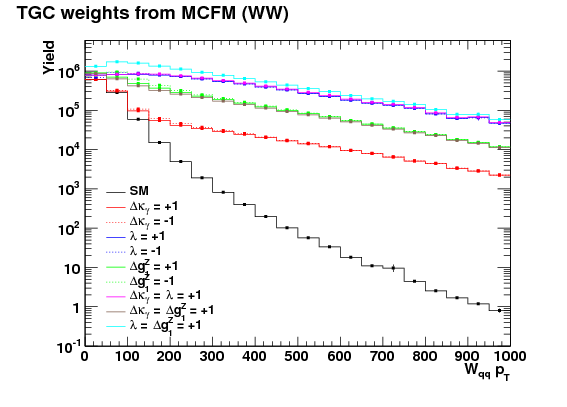
\includegraphics[width=0.48\textwidth]{figs/myfigs/ww-fits.png}
    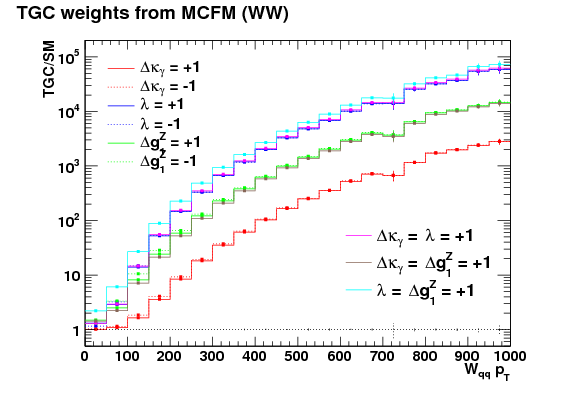
\includegraphics[width=0.48\textwidth]{figs/myfigs/ww-ratios.png} \\
    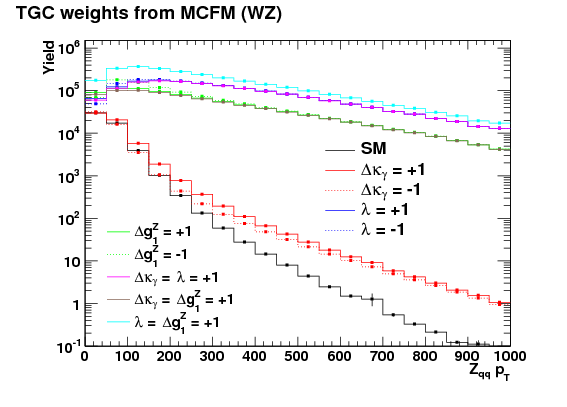
\includegraphics[width=0.48\textwidth]{figs/myfigs/wz-fits.png}
    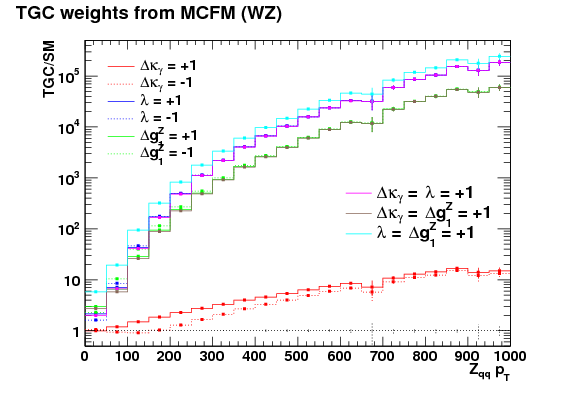
\includegraphics[width=0.48\textwidth]{figs/myfigs/wz-ratios.png} \\
    \caption{The $p_{T}$ distributions of the $q\bar{q}$ system for $WW$ events (top)
    and for $WZ$ events (bottom) at the parton level in the presence of anomalous couplings $\Delta\kappa_{\gamma}$, 
    $\lambda$ and $\Delta{g_{1}^{Z}}$ compared to the SM distribution. Histograms 
    show the absolute contributions for the SM and different ATGC combinations 
    (left) and their deviation relative to the SM prediction (right). The new 
    physics scale is $\Lambda\rightarrow\infty$.}
    \label{fig:kineLEP-ww}}
\end{figure}
%%%%%%%%%%%%%%%%%%%%%%%%%%%%
  We also compare different SM distributions generated with two different 
  generators, \textsc{MadGraph}~\cite{madgraph} and \textsc{MCFM} at LO, as shown in 
  Figure~\ref{fig:wwSMcomparison1} and Figure~\ref{fig:wwSMcomparison2} for 
  $WW\rightarrow \ell\nu{q\bar{q}}$ events. Both generators are using \textsc{CTEQ6L1} 
  PDFs.  For these comparisons, the following cuts were applied at the generator level:
  $|\eta_{q}|<5$, $|\eta_{\bar{q}}|<5$, $|\eta_{\ell}|<2.4$, muon/electron $p_{T}=100-600$~GeV,
  up/down quark $p_{T}>20$~GeV, $\Delta R_{q-\bar{q}}>0.3$, $\Delta R_{lepton-q}>0.3$, 
  $\Delta R_{lepton-\bar{q}}>0.3$, $p_{T}(q\bar{q})>80$~GeV, $M_{q\bar{q}}<160$~GeV, 
  $M_{l\nu}<160$~GeV, and $M_{T}(l\nu)<160$~GeV.
%  (these cuts define the phase space that is used to derive the ATGC weights).  

%%%%%%%%%%%%%%%%%%%%%%%%%%%%
\begin{figure}[h!t]
  {\centering
    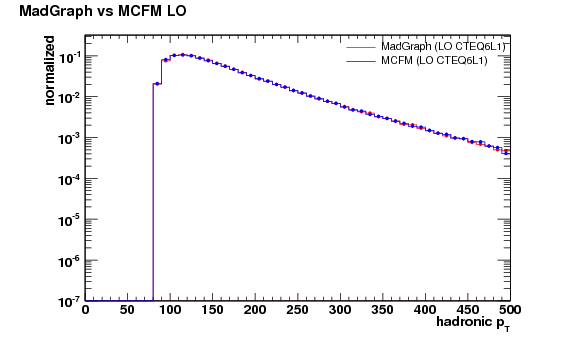
\includegraphics[width=0.48\textwidth]{figs/myfigs/wwComparison62-withCuts-hadronicPt.png}
    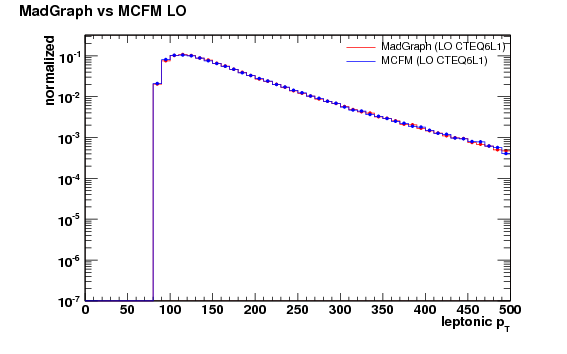
\includegraphics[width=0.48\textwidth]{figs/myfigs/wwComparison62-withCuts-leptonicPt.png} \\
    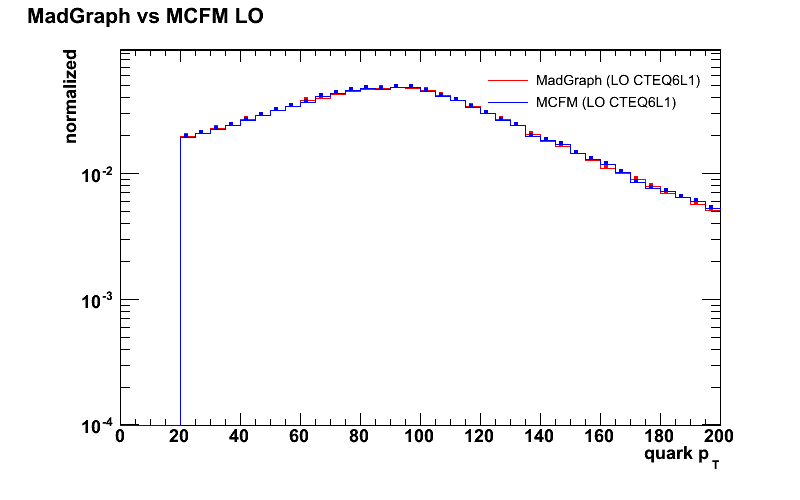
\includegraphics[width=0.48\textwidth]{figs/myfigs/wwComparison62-withCuts-quarkpT.png}
    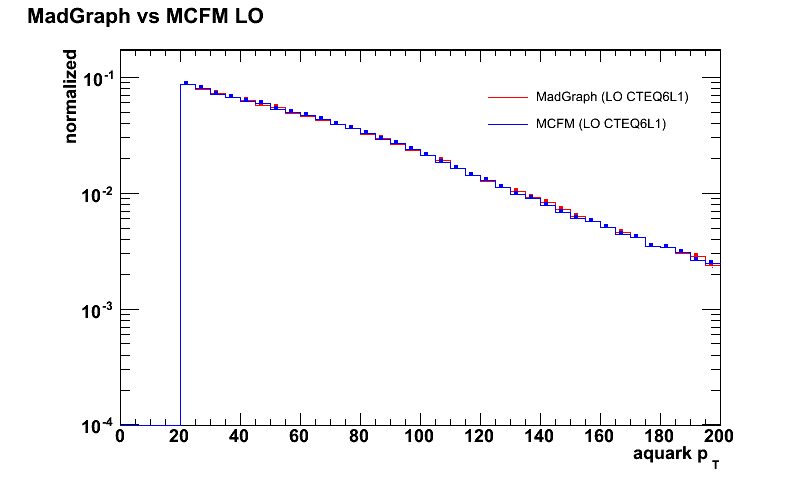
\includegraphics[width=0.48\textwidth]{figs/myfigs/wwComparison62-withCuts-aquarkpT.png} \\
    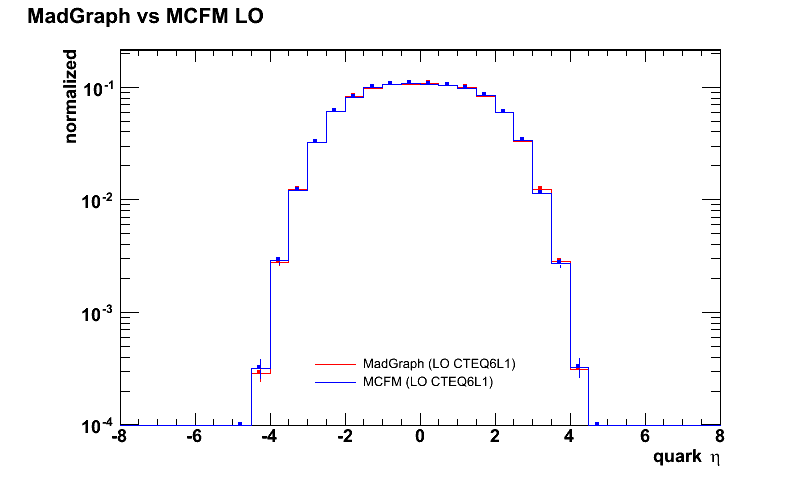
\includegraphics[width=0.48\textwidth]{figs/myfigs/wwComparison62-withCuts-quarkEta.png}
    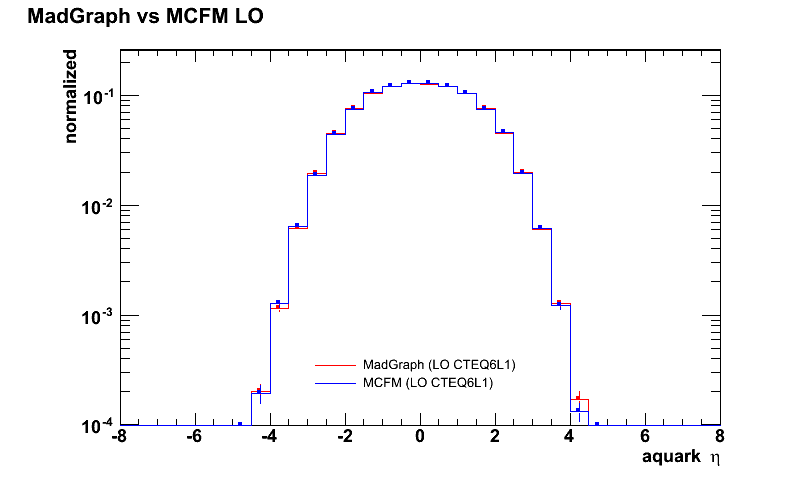
\includegraphics[width=0.48\textwidth]{figs/myfigs/wwComparison62-withCuts-aquarkEta.png} \\
    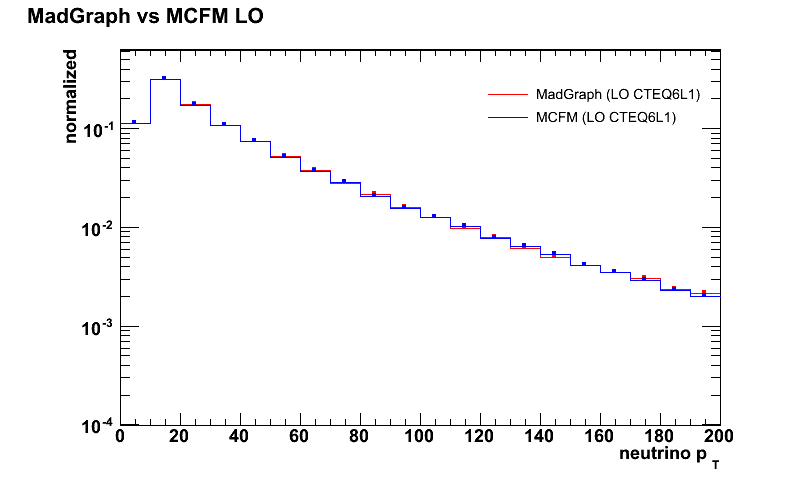
\includegraphics[width=0.48\textwidth]{figs/myfigs/wwComparison62-withCuts-neutrinopT.png}
    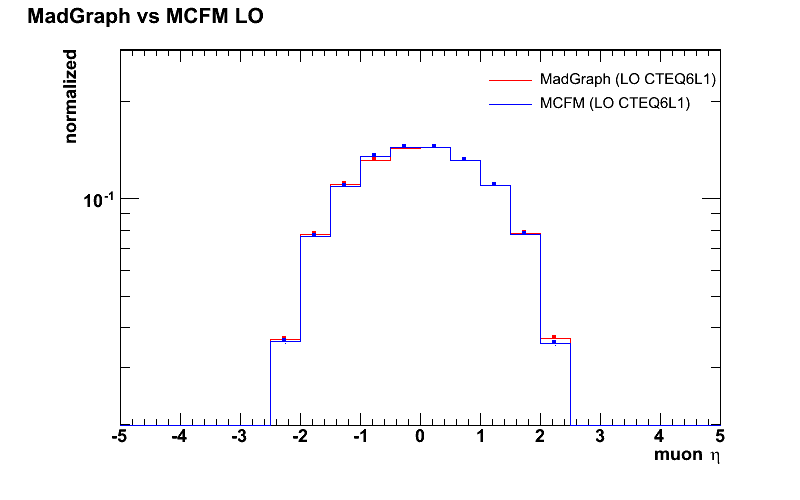
\includegraphics[width=0.48\textwidth]{figs/myfigs/wwComparison62-withCuts-muonEta.png} \\
    \caption{The LO SM distributions of $WW\rightarrow \ell\nu q\bar{q}$ events 
    (\textsc{MadGraph} in red, \textsc{MCFM} in blue). The applied generator 
    level cuts are defined in the text.}
    \label{fig:wwSMcomparison1}}
\end{figure}
%%%%%%%%%%%%%%%%%%%%%%%%%%%%
\begin{figure}[h!t]
  {\centering
    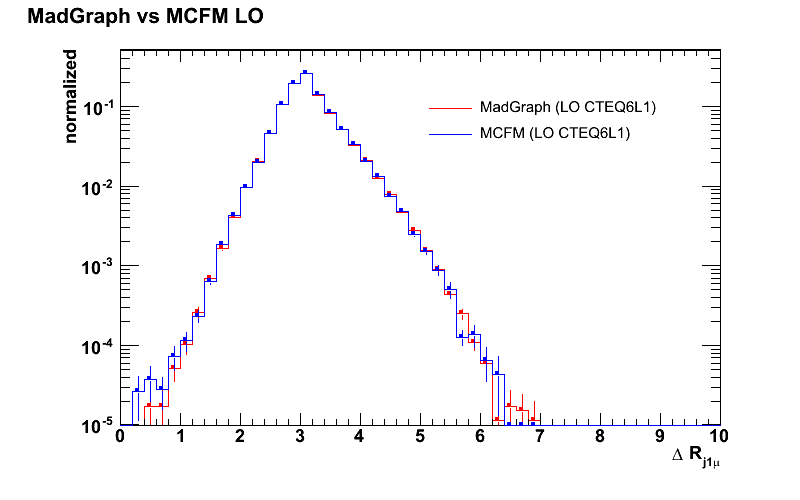
\includegraphics[width=0.48\textwidth]{figs/myfigs/wwComparison62-withCuts-dRmj1.png}
    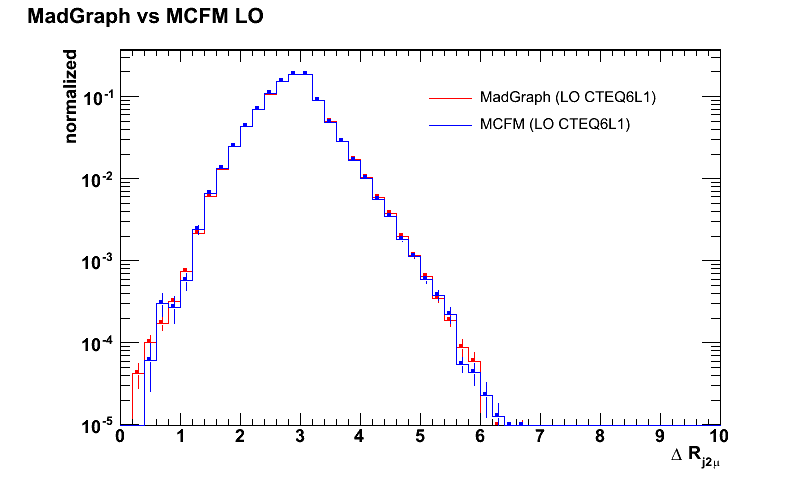
\includegraphics[width=0.48\textwidth]{figs/myfigs/wwComparison62-withCuts-dRmj2.png} \\
    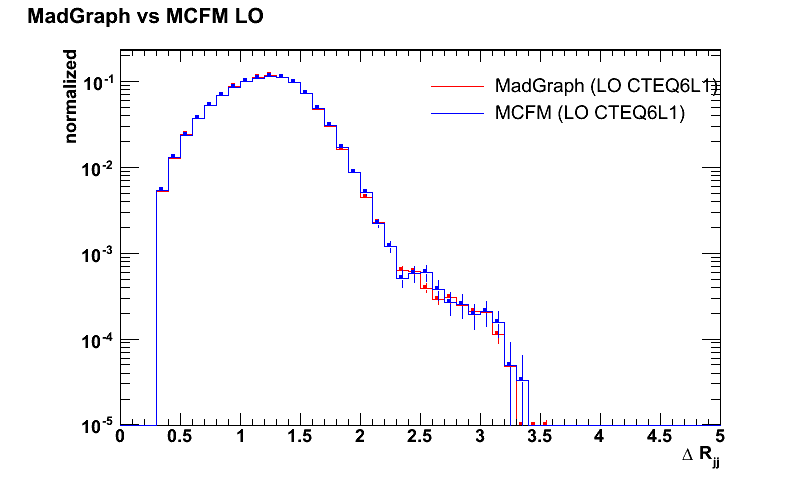
\includegraphics[width=0.48\textwidth]{figs/myfigs/wwComparison62-withCuts-dRjj.png}
    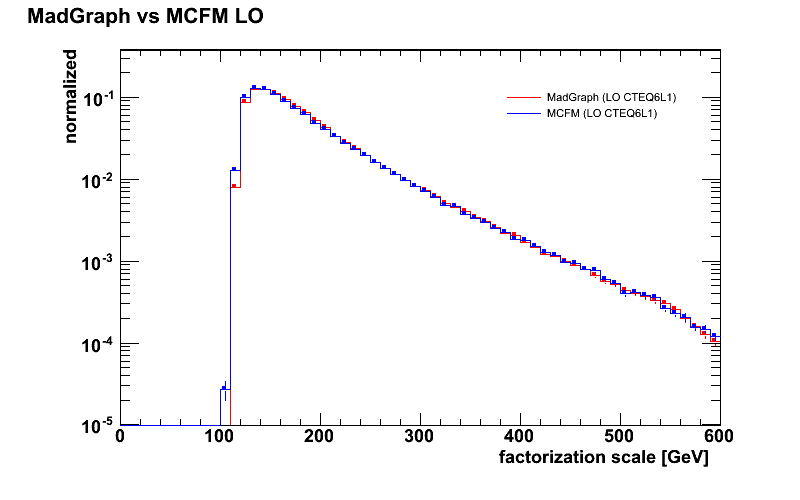
\includegraphics[width=0.48\textwidth]{figs/myfigs/wwComparison62-withCuts-facScale.png} \\
    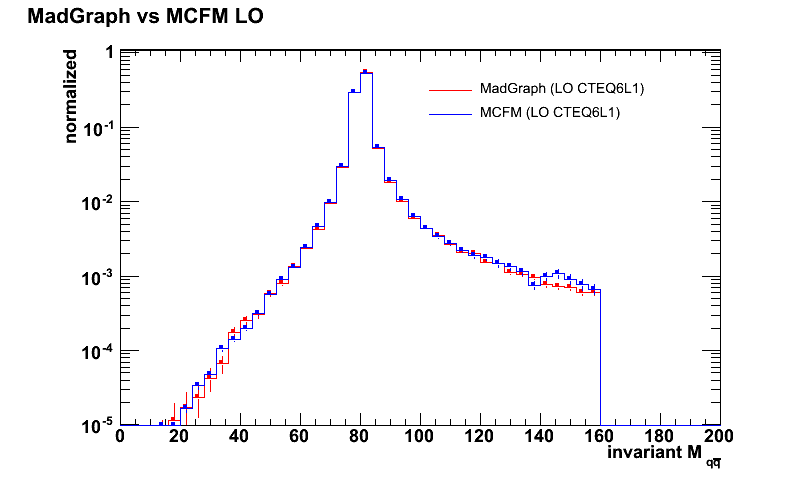
\includegraphics[width=0.48\textwidth]{figs/myfigs/wwComparison62-withCuts-massHadronic.png}
    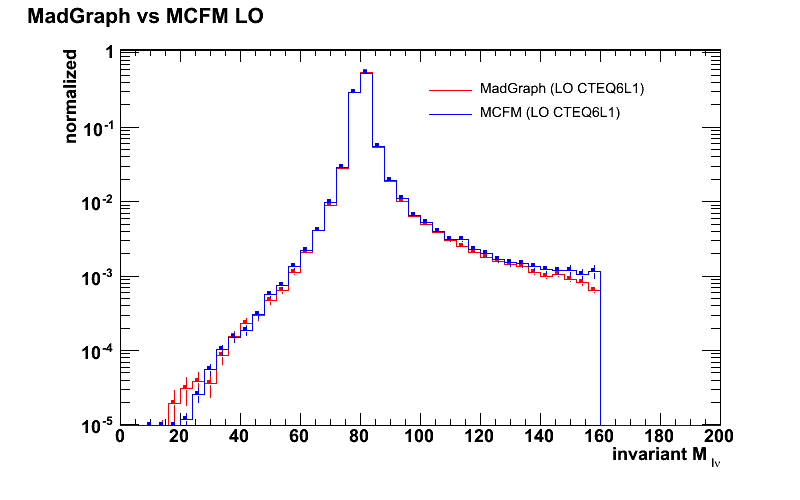
\includegraphics[width=0.48\textwidth]{figs/myfigs/wwComparison62-withCuts-massLeptonic.png} \\
    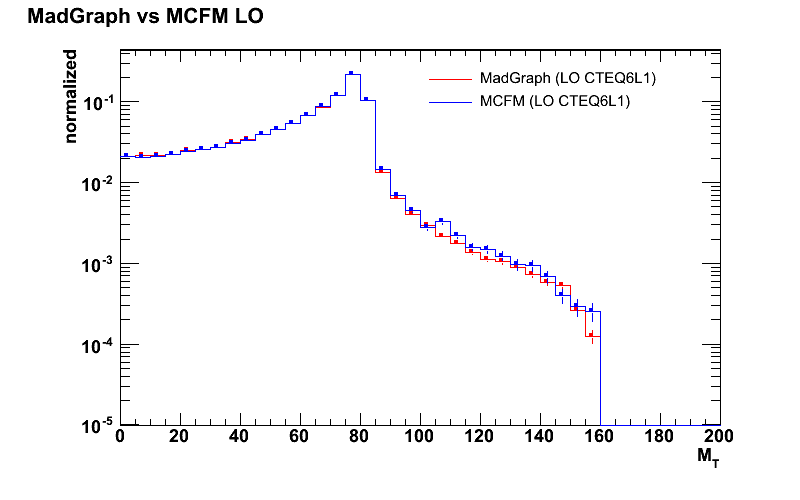
\includegraphics[width=0.48\textwidth]{figs/myfigs/wwComparison62-withCuts-massTrans.png} \\
    \caption{The LO SM distributions of $WW\rightarrow \ell\nu q\bar{q}$ events 
    (\textsc{MadGraph} in red, \textsc{MCFM} in blue). The applied generator 
    level cuts are defined in the text.}
    \label{fig:wwSMcomparison2}}
\end{figure}
%%%%%%%%%%%%%%%%%%%%%%%%%%%%
  The predicted ``anomalous'' cross sections relative to the SM value given 
  by the \textsc{MCFM} generator are shown in Figure~\ref{fig:xSecWW} as a 
  function of anomalous couplings. These cross sections are derived for events 
  selected after applying the generator level cuts similar to those at the 
  reconstructed level for merged jets sample: 
  $|\eta_{\ell}|<2.1$, $|\eta_{q}|<2.4$, $|\eta_{\bar{q}}|<2.4$, $|\eta_{q\bar{q}}|<2.4$,
  $p_{T}(q\bar{q})>200$~GeV, $p_{T}(\ell\nu)>200$~GeV, $\Delta R(\ell-(q\bar{q}))>\pi/2$,
  $\Delta\phi(p_{T}-(q\bar{q}))>2$, $\Delta\phi(p_{T}^{\ell\nu}-(q\bar{q}))>2$, 
  $p_{T}^{\ell}>30$~GeV, $p_{T}^{\nu}>50$~GeV, up/down quark $p_{T}>30$~GeV, 
  $70<M_{q\bar{q}}<100$, $\Delta R_{q-\bar{q}}>0.3$, $\Delta R_{lepton-q}>0.3$, 
  $\Delta R_{lepton-\bar{q}}>0.3$, $M_{l\nu}<160$~GeV, and $M_{T}(l\nu)<160$~GeV.
  We vary only one coupling at the time and 
  keep the other two couplings fixed to their SM values, while respecting the 
  relation~(\ref{eq:lep}). 
%%%%%%%%%%%%%%%%%%%%%%%%%%%%
\begin{figure}[h!t]
  {\centering
    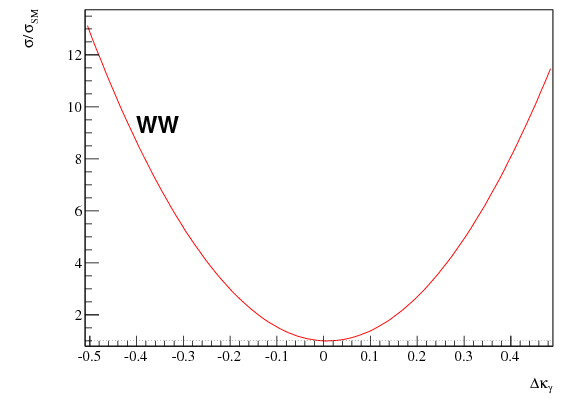
\includegraphics[width=0.48\textwidth]{figs/myfigs/ww-xsection-kappa.png}
    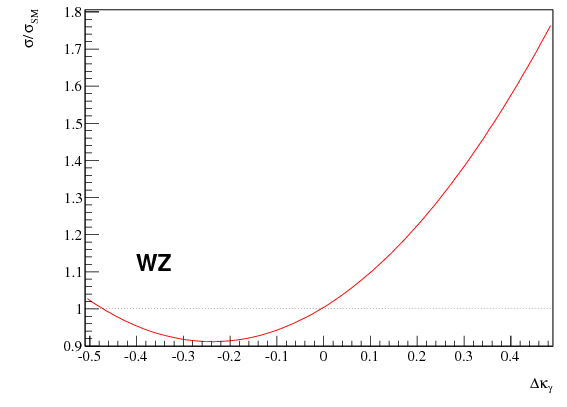
\includegraphics[width=0.48\textwidth]{figs/myfigs/wz-xsection-kappa.png} \\
    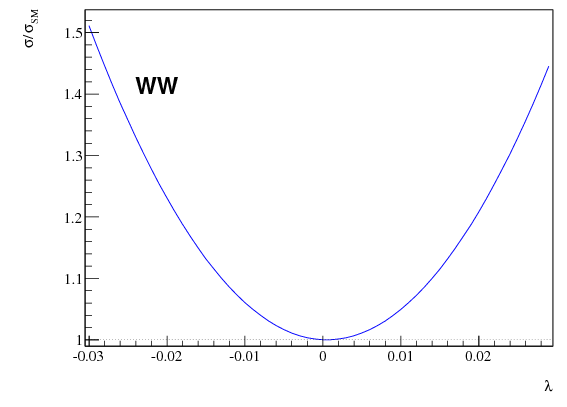
\includegraphics[width=0.48\textwidth]{figs/myfigs/ww-xsection-lambda.png} 
    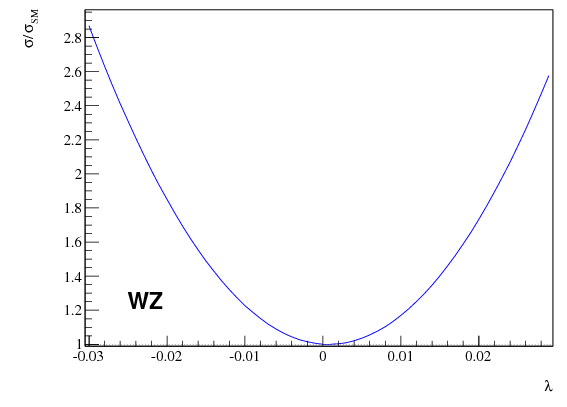
\includegraphics[width=0.48\textwidth]{figs/myfigs/wz-xsection-lambda.png} \\ 
    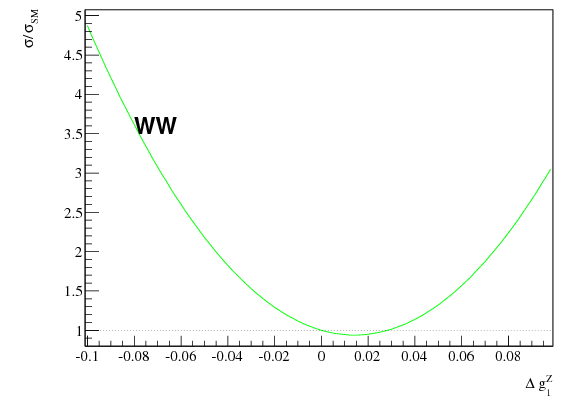
\includegraphics[width=0.48\textwidth]{figs/myfigs/ww-xsection-g1z.png}
    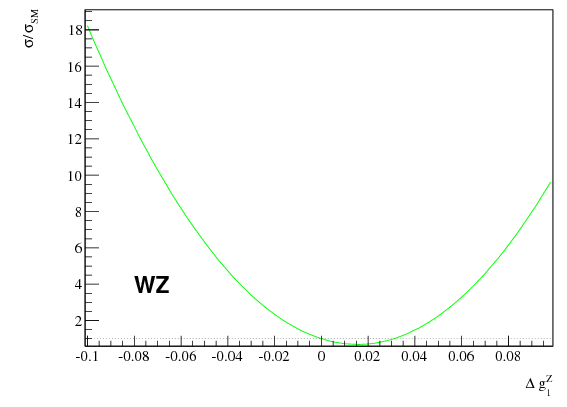
\includegraphics[width=0.48\textwidth]{figs/myfigs/wz-xsection-g1z.png} \\
    \caption{Production cross sections for $WW\rightarrow \ell\nu q\bar{q}$ (left) 
    and $WZ\rightarrow \ell\nu q\bar{q}$ (right) normalized to the SM prediction 
    as a function of anomalous couplings 
    $\Delta\kappa_{\gamma}$ ($\lambda = \Delta{g_{1}^{Z}}=0$) (top),  
    $\lambda$ ($\Delta\kappa_{\gamma}=\Delta{g_{1}^{Z}}=0$) (middle), and 
    $\Delta{g_{1}^{Z}}$ ($\Delta\kappa_{\gamma}=\lambda=0$) (bottom).}
    \label{fig:xSecWW}}
\end{figure}
%%%%%%%%%%%%%%%%%%%%%%%%%%%%
%%%%%%%%%%%%%%%%%%%%%%%%%%%%
%  \subsection{Monte Carlo Modeling of Anomalous TGCs}
%  \label{sec:reweight}
%  \noindent
  \par
  To estimate the sensitivity of the measurement of anomalous couplings $\kappa_{\gamma}, 
  \lambda$ and $g_{1}^{Z}$ and measure their values in data we compare data to 
  MC predictions with different ATGC values (ATGC grid). The ATGC grid is constructed 
  by reweighting the SM a\textsc{MC@NLO} events to different \textsc{MCFM} predictions 
  in the presence of ATGCs.  The reweighting method uses the calculated matrix element 
  values to predict the rate with which a given event would be generated if there would 
  be an anomalous coupling present.  The idea of using this method is to assign to each 
  a\textsc{MC@NLO} SM event an additional weight (derived at the generator level) which 
  is a function of anomalous couplings and predicts the change in event rate if its value 
  differs from the SM prediction.  The calculated weight represents a ratio of squared 
  matrix elements with and without the anomalous coupling i.e., 
  $|{\mathcal M}|^{2}/|{\mathcal M}|_{SM}^{2}$, where $|{\mathcal M}|^{2}$ is the matrix 
  element squared in the presence of anomalous couplings and $|{\mathcal M}|_{SM}^{2}$ is 
  the matrix element squared in the SM.  Because in the SM 
  $\Delta\kappa_{V}=\lambda=\Delta g_{1}^{V}=0$, an event weight is equal to 1 
  and does not change the event rate.  Ideally, after applying these weights, particles' 
  4-vectors in that event are ``modified'' (reweighted) to correspond to the analogous ATGC 
  case.  The basis of this method is that the equation of the differential cross section, 
  which has a quadratic dependence on ATGCs can be written as:
%  \begin{equation}
%  \begin{array}{ccl}
%  d\sigma & = & {\textit{const}}\cdot|\mathcal M|^{2}dX \\ 
%  & = & {\textit{const}}\cdot|\mathcal M|_{SM}^{2}\frac{|{\mathcal M}|^{2}}{|{\mathcal M}|_{SM}^{2}}dX \\
%  & = & {\textit{const}}\cdot|\mathcal M|^{2}_{SM}[1+A(X)\Delta\kappa+B(X)\Delta\kappa^{2}+
%   C(X)\Delta\lambda+D(X)\Delta\lambda^{2}+E(X)\Delta\kappa\Delta\lambda + ...]dX \\
%  & = & d\sigma_{SM}\cdot R(X;\Delta\kappa,\Delta\lambda, ...)
%  \label{eq:expan}
%  \end{array}{}
%  \end{equation}
  \begin{equation}
    \begin{array}{ccl} d\sigma & \propto & |\mathcal M|^{2}dx \\ & \propto & |\mathcal
      M|_{SM}^{2}\frac{|{\mathcal M}|^{2}}{|{\mathcal M}|_{SM}^{2}}dx \\ &
      \propto & |\mathcal M|^{2}_{SM}[1+A\Delta\kappa+B(\Delta\kappa)^{2} + C\lambda + 
      D\lambda^{2}+E\Delta g_{1}+F(\Delta g_{1})^{2} \\ &
      + & G\Delta\kappa\lambda + H\Delta\kappa\Delta g_{1}+I\lambda\Delta g_{1}]dx \\ & 
      \propto & d\sigma_{SM}\cdot R(\Delta\kappa,\lambda,\Delta g_{1}),  
        \label{eq:expan} 
    \end{array}{} 
  \end{equation}
  where $d\sigma$ is the differential cross section which includes the contribution 
  from the anomalous couplings, $d\sigma_{SM}$ is the SM differential cross section, 
  $X$ is a kinematic distribution sensitive to the anomalous couplings ($p_{T}^{q\bar{q}}$ 
  in our case), and $A,B,C,D,E,F,G,H$ and $I$ are reweighting coefficients dependent 
  on event kinematics, $X$. Then the weight $R$ represents the ratio of matrix elements 
  squared, $|{\mathcal M}|^{2}/|{\mathcal M}|_{SM}^{2}$, and it is calculated for each 
  event depending on the set of $X$-variables and ATGCs as:
  \begin{equation}
  \begin{array}{ccl}
  & R(X;\Delta\kappa,\lambda,\Delta g_{1}) = 
  1+A(X)\Delta\kappa+B(X)\Delta\kappa^{2}+C(X)\lambda+D(X)\lambda^{2}+
  E(X)\Delta g_{1} \\
  &+F(X)\Delta g_{1}^{2} + G(X)\Delta\kappa\lambda+H(X)\Delta\kappa \Delta g_{1}+
  I(X)\lambda\Delta g_{1} \\
  \label{eq:expan2}
  \end{array}{}
  \end{equation}
  where $\Delta\kappa=\Delta\kappa_{\gamma}$ and $\Delta{g_{1}}=\Delta{g_{1}^{Z}}$.  
  The SM differential distribution $X$, weighted by $R(X;\Delta\kappa,\lambda,\Delta g_{1})$ 
  describes the kinematic distributions $X$ in the presence of a non-SM coupling $\kappa,
  \lambda$ and/or $g_{1}^{Z}$.  Depending on the number of reweighting coefficients, 
  the system of the same number of equations allow us to calculate their values which 
  are unique for each event.  Having 3 independent couplings $\kappa, \lambda$ and $g_{1}$ 
  we can decompose the expression given by Eq.~(\ref{eq:expan2}) as:
  \begin{equation}
  \begin{array}{ccl}
  R_{1} & = & 1+C\mid{\lambda}\mid+D\mid{\lambda}^{2}\mid \\
  R_{2} & = & 1-C\mid{\lambda}\mid+D\mid{\lambda}^{2}\mid \\
  R_{3} & = & 1+A\mid{\Delta}{\kappa}\mid+B\mid{\Delta}{\kappa}^{2}\mid \\
  R_{4} & = & 1-A\mid{\Delta}{\kappa}\mid+B\mid{{{\Delta}{\kappa}}^{2}\mid} \\
  R_{5} & = & 1+E\mid{\Delta}{g_{1}}\mid+F\mid{\Delta}{g_{1}}^{2}\mid \\
  R_{6} & = & 1-E\mid{\Delta}{g_{1}}\mid+F\mid{{{\Delta}{g_{1}}}^{2}\mid} \\
  R_{7} & = & 1+A\mid{\Delta}{\kappa}\mid+B\mid{{{\Delta}{\kappa}}^{2}\mid}+
                C\mid{\lambda}\mid+D\mid{{{\lambda}}^{2}\mid}+
                G\mid{\Delta}{\kappa}\mid\mid{\lambda}\mid \\
  R_{8} & = & 1+A\mid{\Delta}{\kappa}\mid+B\mid{{{\Delta}{\kappa}}^{2}\mid}+
                E\mid{\Delta{g_{1}}}\mid+F\mid{{{\Delta{g_{1}}}}^{2}\mid}+
                H\mid{\Delta}{\kappa}\mid\mid{\Delta{g_{1}}}\mid \\
  R_{9} & = & 1+C\mid{\lambda}\mid+D\mid{{{\lambda}}^{2}\mid}+
                E\mid{\Delta{g_{1}}}\mid+F\mid{{{\Delta{g_{1}}}}^{2}\mid}+
                I\mid{\lambda}\mid\mid{\Delta{g_{1}}}\mid
  \label{eq:arovi}
  \end{array}{}
  \end{equation}
  where $R_{1-9}$ are $|{\mathcal M}|^{2}/|{\mathcal M}|_{SM}^{2}$ ratios for a 
  chosen set of couplings, ${\Delta}{\kappa}={\Delta\kappa_{\gamma}}$, and 
  $\Delta{g_{1}}=\Delta{g_{1}^{Z}}$.  Due to the electro-magnetic invariance, 
  $g_{1}^{\gamma}$ is fixed to its SM value of 1.  The values of 
  ${\Delta}{\kappa},\lambda$ and $\Delta{g_{1}}$ couplings are arbitrarily chosen 
  to be $|\Delta\kappa_{\gamma}|=|\lambda|=|\Delta{g_{1}^{Z}}|=1$ 
  as presented in Table~\ref{tab:set1}.  

  \begin{table}[htb]
  \begin{center}
  \begin{tabular}{|c|c|c|c|c|c|c|c|c|c|} \hline
  & \multicolumn{9}{c|}{``ATGC parametrization''} \\ \hline \hline
  & $R_1$& $R_2$& $R_3$& $R_4$& $R_5$& $R_6$& $R_7$& $R_8$& $R_9$ \\ \hline
  $\Delta\kappa_{\gamma}$ & 0 & 0 & +1.0 & -1.0 & 0 & 0 & +1.0 & +1.0 & 0 \\ \hline
  $\lambda$ & +1.0 & -1.0& 0 & 0 & 0 & 0 & +1.0 & 0 & +1.0 \\ \hline
  $\Delta{g_{1}^{Z}}$ & 0 & 0 & 0 & 0 & +1.0 & -1.0 & 0 & +1.0 & +1.0 \\ \hline
  \end{tabular}
  \end{center}
  \caption{The values of $\Delta\kappa_{\gamma}$, $\lambda$ and 
  $\Delta{g_{1}^{Z}}$ used to calculate the reweighting coefficients $A,B,C,D,E,
  F,G,H$ and $I$ with $\Lambda\rightarrow\infty$ (relation given by 
  Eq.~(\ref{eq:lep}) allows us to calculate $\Delta\kappa_{Z}$ for given 
  $\Delta\kappa_{\gamma}$ and $\Delta{g_{1}^{Z}}$ values.}
  \label{tab:set1}
  \end{table}
  %
  The values of $R_{1-9}$ are the exact values given by a generator where matrix 
  element $|{\mathcal M}|^{2}$ with ATGC contribution, is recalculated using the same 
  4-vectors as for $|{\mathcal M}|^{2}_{SM}$ (\mcfm\ generator is adapted by authors 
  to recalculate $|{\mathcal M}|^{2}$ based on the SM 4-vectors).  The reweighting 
  coefficients can be calculated for each event from Eq.~(\ref{eq:arovi}) as:
  \begin{equation}
  \begin{array}{ccl}
  C & = & (R_{1}-R_{2})/2\lambda \\
  D & = & (R_{1}+R_{2}-2)/2\lambda^{2}\\
  A & = & (R_{3}-R_{4})/2\Delta\kappa_{\gamma} \\
  B & = & (R_{3}+R_{4}-2)/2\Delta\kappa_{\gamma}^{2} \\
  E & = & (R_{5}-R_{6})/2\Delta{g_{1}^{Z}} \\
  F & = & (R_{5}+R_{6}-2)/2\Delta{g_{1}^{Z}}^{2} \\
  G & = & (R_{7}-1-A\Delta\kappa_{\gamma}-B\Delta\kappa_{\gamma}^{2}-
  C\lambda-D\lambda^{2})/\Delta\kappa_{\gamma}\lambda \\
  H & = & (R_{8}-1-A\Delta\kappa_{\gamma}-B\Delta\kappa_{\gamma}^{2}-
  E\Delta{g_{1}^{Z}}-F\Delta{g_{1}^{Z}}^{2})/\Delta\kappa_{\gamma}\Delta{g_{1}^{Z}} \\
  I & = & (R_{9}-1-C\lambda-D\lambda^{2}-
  E\Delta{g_{1}^{Z}}-F\Delta{g_{1}^{Z}}^{2})/\lambda\Delta{g_{1}^{Z}},
  \label{eq:coeff}
  \end{array}{}
  \end{equation}
  by setting $|\Delta\kappa_{\gamma}|=|\lambda|=|\Delta{g_{1}^{Z}}|=1$.  
  The coefficients $A-I$ are functions of kinematic variable $X$.  Plugging these 
  coefficients back into Eq.~(\ref{eq:arovi}), we can calculate the weight $R$ for 
  any arbitrary choice of $\Delta\kappa_{\gamma}$, $\lambda$ and/or 
  $\Delta{g_{1}^{Z}}$.  The \textsc{MCFM} SM distributions weighted by $R$ per event 
  will produce that same distribution as it would be predicted by the \textsc{MCFM} 
  generator in the presence of the same ATGCs. Comparison between the reweighted 
  \mcfm\ distributions to those obtained with the \textsc{VBF@NLO} generator are 
  shown in Figure~\ref{fig:rewWW}.  
%  Because we are 
%  reweighting the SM \textsc{MadGraph} distributions (at the generator level on an 
%  event-by-event basis) using the predictions from \textsc{MCFM} in the presence of 
%  ATGCs, we have to map events from these two generators based on event kinematics 
%  (now here say how they super agree ...).  

%%%%%%%%%%%%%%%%%%%%%%%%%%%%
\begin{figure}[h!t]
  {\centering
    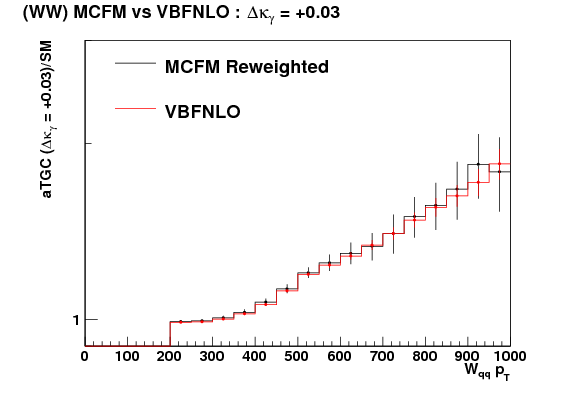
\includegraphics[width=0.48\textwidth]{figs/myfigs/ww-kappa-ratio.png}
    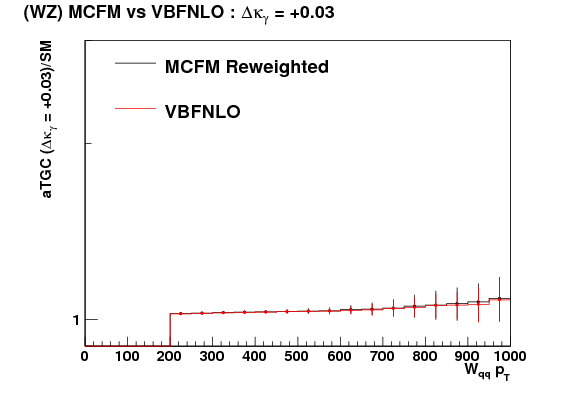
\includegraphics[width=0.48\textwidth]{figs/myfigs/wz-kappa-ratio.png} \\
    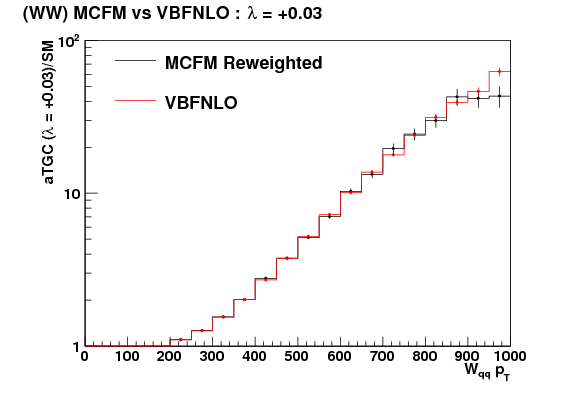
\includegraphics[width=0.48\textwidth]{figs/myfigs/ww-lambda-ratio.png} 
    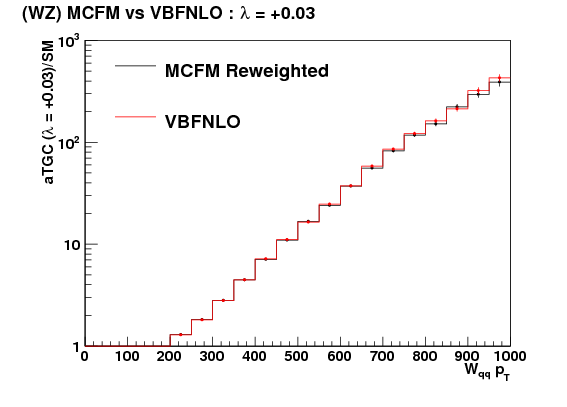
\includegraphics[width=0.48\textwidth]{figs/myfigs/wz-lambda-ratio.png} \\
    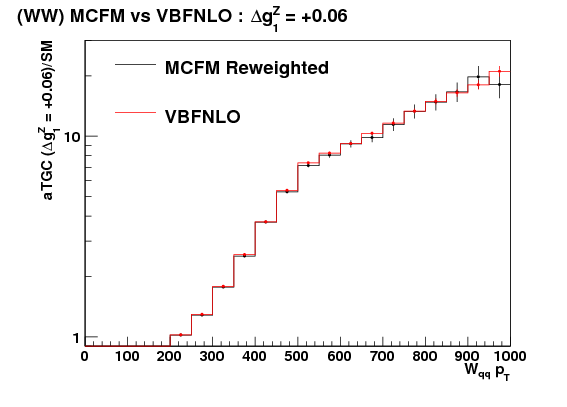
\includegraphics[width=0.48\textwidth]{figs/myfigs/ww-g1z-ratio.png}
    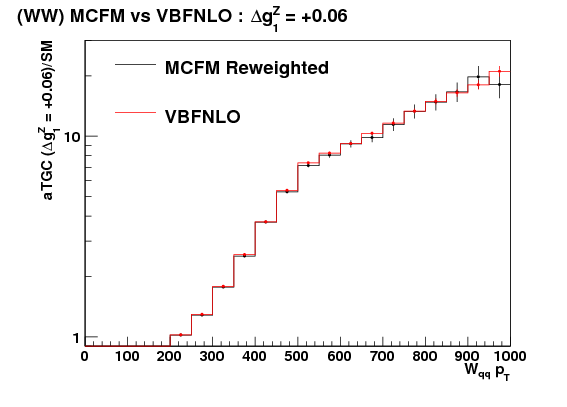
\includegraphics[width=0.48\textwidth]{figs/myfigs/ww-g1z-ratio.png} \\
    \caption{The comparison of \textsc{MCFM} $p_{T}^{q\bar{q}}$ distributions explicitly 
    predicted by the generator (solid line) and those reweighted to distributions in the 
    presence of anomalous couplings (dashed line).}
    \label{fig:rewWW}}
\end{figure}
%%%%%%%%%%%%%%%%%%%%%%%%%%%%

\par
Using the analytical expression given by Eq.~(\ref{eq:arovi}), the ATGC samples 
were produced with a large set of ATGC parameters: for $|\Delta\kappa_{\gamma}|\leq~0.15$ 
in steps of $\Delta\kappa_{\gamma}=0.01$, $|\lambda|\leq~0.03$ in steps of 
$\lambda=0.001$, and $|\Delta{g_{1}^{Z}}|\leq~0.10$ in steps of $\Delta{g_{1}^{Z}}=0.002$. 
Figure~\ref{fig:ww_dijetPt_atgcRatio} shows the ratios of hadronic $W/Z$ $p_T$ 
spectra relative to the SM for various values of ATGCs. 
%%%%%%%%%%%%%%%%%%%%%%%%%%%%
\begin{figure}[h!t]
  {\centering
    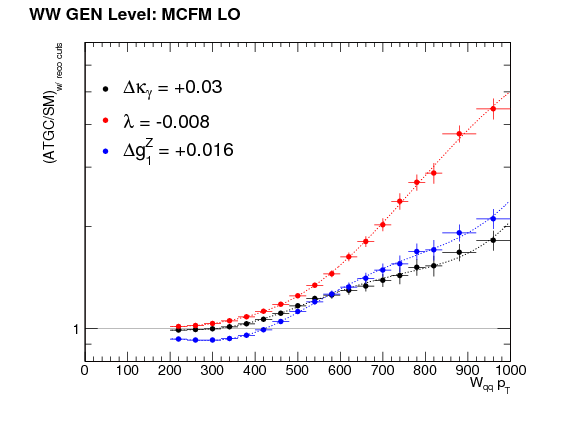
\includegraphics[width=0.48\textwidth]{figs/myfigs/ww-mix-fitFunctions1D.png}
    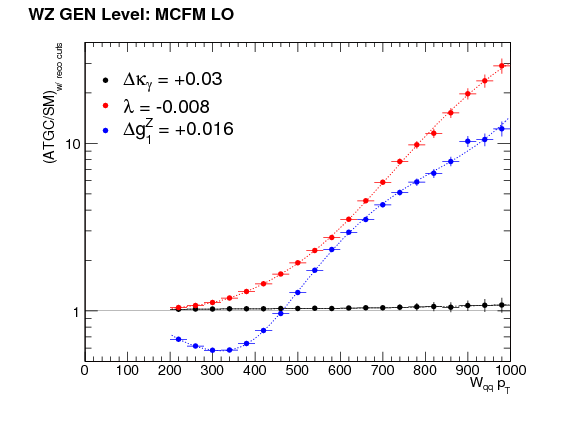
\includegraphics[width=0.48\textwidth]{figs/myfigs/wz-mix-fitFunctions1D.png} \\
    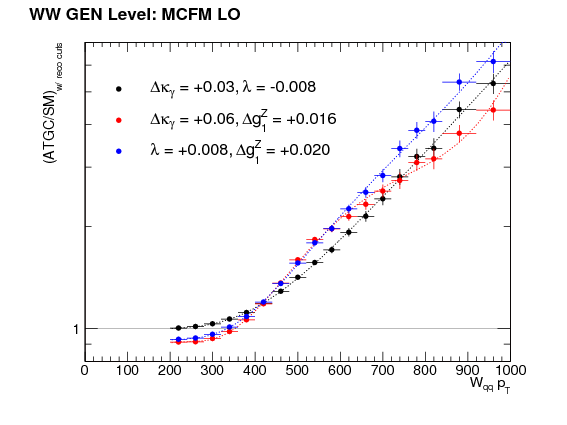
\includegraphics[width=0.48\textwidth]{figs/myfigs/ww-mix-fitFunctions2D.png}
    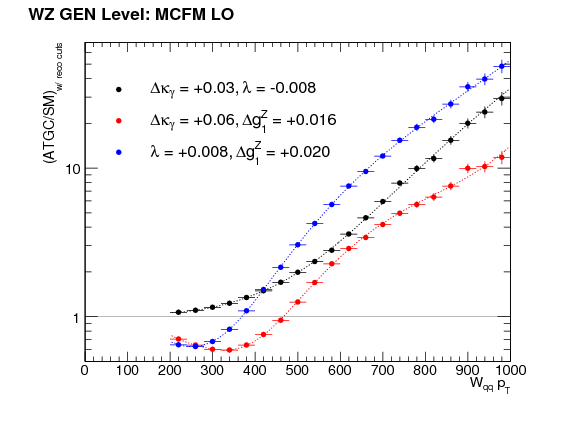
\includegraphics[width=0.48\textwidth]{figs/myfigs/wz-mix-fitFunctions2D.png} \\
    \caption{Ratio of the hadronic $W$ (left) and $Z$ (right) $p_T$ distributions 
    for various anomalous coupling values relative to the standard model coupling 
    fitted with a polynomial function.}
    \label{fig:ww_dijetPt_atgcRatio}}
\end{figure}
%%%%%%%%%%%%%%%%%%%%%%%%%%%%
In order to obtain predictions for a continuous variation in ATGC parameter 
values as a function of hadronic $q\bar{q}$ $p_T$, we parametrize the above 
ratios using following polynomial functions for $WW$ distributions: 
%%%%%%%%%%%
\begin{equation}
% [0]+x*([1]+x*([2]+x*([3]+x*([4]+x*[5]))))
\text{Ratio} = p_{0}+p_{1}\cdot{x}+p_{2}\cdot{x}^{2}+p_{3}\cdot{x}^{3}+p_{4}\cdot{x}^{4}+p_{5}\cdot{x}^{5},
\label{eqatgcparam}
\end{equation}
and for $WZ$ distributions:
\begin{equation}
% [0]+x*([1]+x*([2]+x*([3]+x*x*([4]+x*([5])))))
% [0]+x*([1]+x*([2]+x*([3]+x*([4]+x*([5]+x*([6]))))))
\text{Ratio}(\Delta\kappa_{\gamma}-\lambda) = 
p_{0}+p_{1}\cdot{x}+p_{2}\cdot{x}^{2}+p_{3}\cdot{x}^{3}+p_{4}\cdot{x}^{5}+p_{5}\cdot{x}^{6},  
\label{eqatgcparam1}
\end{equation}
\begin{equation}
\text{Ratio}(\Delta\kappa_{\gamma}-\Delta g_{1}^{Z};\lambda-\Delta g_{1}^{Z}) = 
p_{0}+p_{1}\cdot{x}+p_{2}\cdot{x}^{2}+p_{3}\cdot{x}^{3}+p_{4}\cdot{x}^{4}+p_{5}\cdot{x}^{5}+p_{6}\cdot{x}^{6}, 
\label{eqatgcparam2}
\end{equation}


%%%%%%%%%%%
where the variable $x$ is hadronic $W/Z$ $p_T$ and the fit parameters $p_{i}$ ($i=0-6$) 
are functions of the anomalous couplings. This function is used later to account for 
the ATGC signal change relative to the SM when fitting the MC ATGC grid points to data. 
The fit parameters as a function of anomalous couplings are shown in Figure~\ref{fig:wwParams} 
and Figure~\ref{fig:wzParams}.
%%%%%%%%%%%%%%%%%%%%%%%%%%%%
\begin{figure}[h!t]
  {\centering
    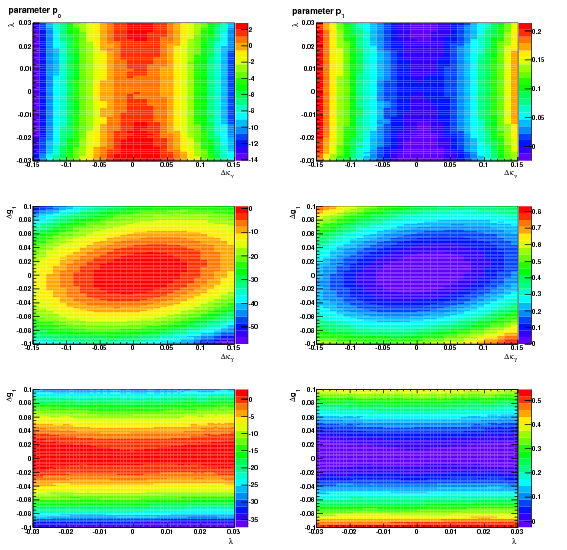
\includegraphics[width=0.48\textwidth]{figs/myfigs/ww-coefficients-1.png}
    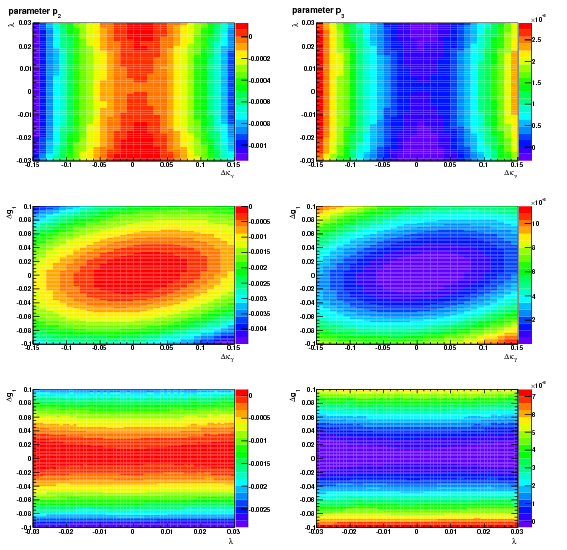
\includegraphics[width=0.48\textwidth]{figs/myfigs/ww-coefficients-2.png} \\
    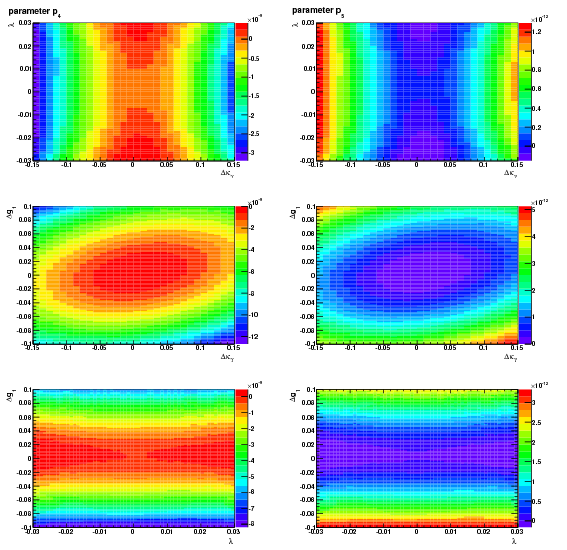
\includegraphics[width=0.48\textwidth]{figs/myfigs/ww-coefficients-3.png}
    \caption{The fit parameters as a function of anomalous couplings for $WW$ 
    distributions.}
    \label{fig:wwParams}}
\end{figure}
%%%%%%%%%%%%%%%%%%%%%%%%%%%%
\begin{figure}[h!t]
  {\centering
    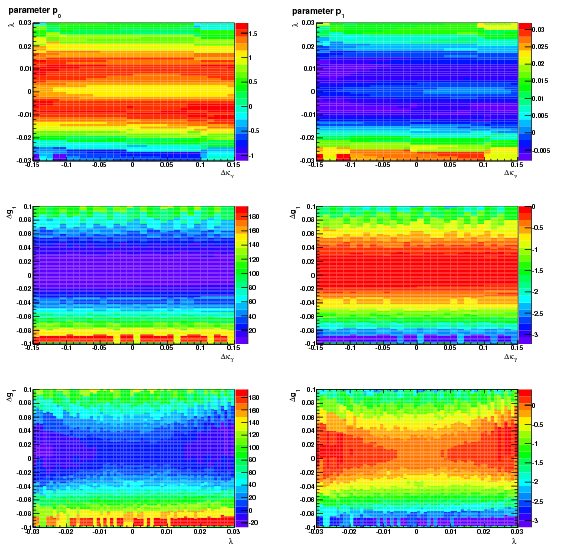
\includegraphics[width=0.48\textwidth]{figs/myfigs/wz-coefficients-1.png}
    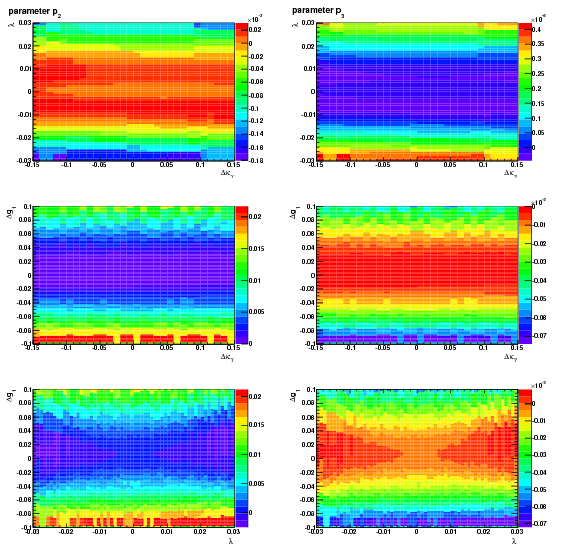
\includegraphics[width=0.48\textwidth]{figs/myfigs/wz-coefficients-2.png} \\
    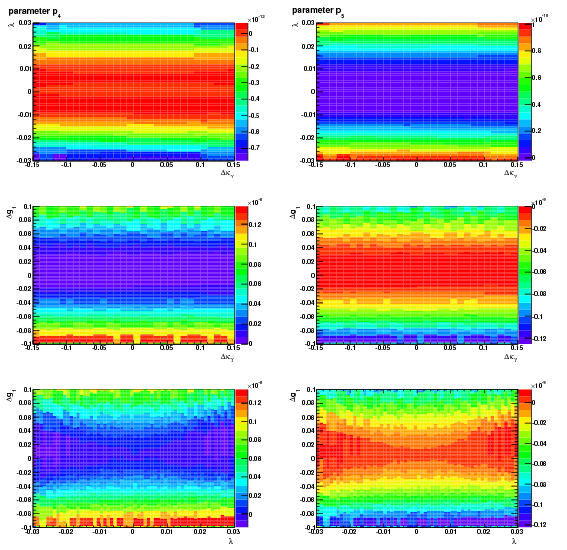
\includegraphics[width=0.48\textwidth]{figs/myfigs/wz-coefficients-3.png}
    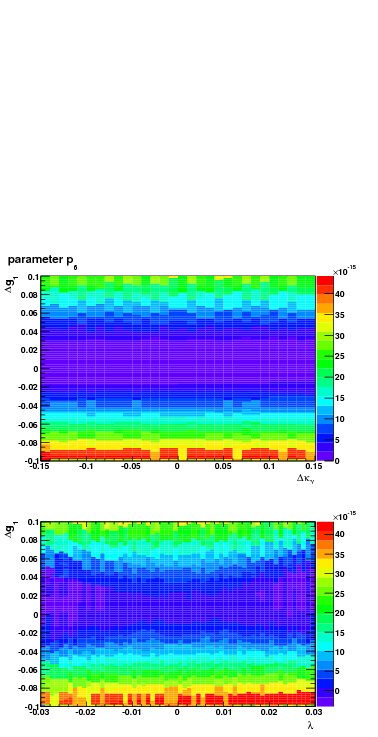
\includegraphics[width=0.23\textwidth]{figs/myfigs/wz-coefficients-4.png} \\
    \caption{The fit parameters as a function of anomalous couplings for $WZ$ 
    distributions.}
    \label{fig:wzParams}}
\end{figure}
%%%%%%%%%%%%%%%%%%%%%%%%%%%%


%%%%%%%%%%%
%\begin{eqnarray}
%\text{Ratio} (\lambda_Z) &=& C_0 (\lambda_Z)  + C_1 (\lambda_Z) \cdot p_T
%                           + C_2 (\lambda_Z) \cdot p_T^2,  \nonumber \\
%\text{Ratio} (\Delta{\kappa_\gamma}) &=& C'_0 (\Delta{\kappa_\gamma})  + 
%                      C'_1 (\Delta{\kappa_\gamma}) \cdot p_T + 
%                      C'_2 (\Delta{\kappa_\gamma}) \cdot p_T^2,  \nonumber \\
%\text{Ratio} (\Delta{g_1^Z}) &=& C''_0 (\Delta{g_1^Z})  + C''_1 (\Delta{g_1^Z}) \cdot p_T
%                           + C''_2 (\Delta{g_1^Z}) \cdot p_T^2, 
%\end{eqnarray}
%%%%%%%%%%%
%where 
%%%%%%%%%%%
%\begin{eqnarray}
%C_i (\lambda_Z) &=& P_{i0} + P_{i1} \cdot \lambda_Z + P_{i2} \cdot \lambda_Z^2, \nonumber \\
%C_i (\Delta{\kappa_\gamma}) &=& P'_{i0} + P'_{i1} \cdot \Delta{\kappa_\gamma} + P'_{i2} \cdot \Delta{\kappa_\gamma}^2, \nonumber \\
%C_i (\Delta{g_1^Z}) &=&  P''_{i0} + P''_{i1} \cdot \Delta{g_1^Z} + P''_{i2} \cdot {\Delta{g_1^Z}}^2,
%\end{eqnarray}
%%%%%%%%%%%
%where $P_{ij}$, $P'_{ij}$, and $P''_{ij}$ are constant parameters. 
%Indices $i, j = 0, 1, 2$. The linear terms $C_1, C'_1, C''_1$ turn out 
%to be zero in all cases. 
%Figure~\ref{fig:ww_dijetPt_aTGC_parametrization} shows the parametrization.



\clearpage
%%%%%%%%%%%%%%%%%%%%%%%%%%%%
\subsection{Existing limits}
The current best fit results for anomalous couplings are dominated by LEP 
results. Table~\ref{tab:aTGC_limits_fromPDG} shows the existing limits for 
various couplings including the best limits from the Tevatron 
experiments~\cite{cdf,d0tgc}. Recent LHC measurements in the fully leptonic 
final state ($WW\to\ell^+\nu\ell^-\overline{\nu}$) are approaching similar 
sensitivity~\cite{Chatrchyan:2011tz,Aad:2012ks}.
%%%%%%%%%%%%%%%%%%%%%%%%%%%%%
\begin{table}[h]
\caption{\label{tab:aTGC_limits_fromPDG}
Current 68\% and 95\% C.L. limits on anomalous couplings. The world best 
limits are based on a fit of LEP measurements (68\% C.L.). The LHC and 
Tevatron 95\% C.L. limits are shown for comparison.}
\begin{center}
  \begin{tabular}{l c}
    \hline  \hline
   Coupling  &  Particle Data Group Fit (68\% C.L.) \\\hline
   $\lambda_\gamma$  &  $0.028^{+0.020}_{- 0.021}$ \\
   $\lambda_Z$  &  $0.088^{+0.060}_{- 0.057}$ \\
   $\Delta{g_1^Z}$  &  $0.016^{+0.022}_{- 0.019}$ \\
   $\Delta{\kappa_\gamma}$  &  $0.027^{+0.044}_{- 0.045}$ \\
   $\Delta{\kappa_Z}$  &  $0.026^{+0.059}_{- 0.056}$ \\
    \hline  
\end{tabular}
\vskip 2mm
%%%%%%
  \begin{tabular}{l c c}
   \hline  
Coupling & D0 ($WW +WZ\to\ell\nu{jj}$) / Combination & CDF ($WW\to\ell^+\nu\ell^-\overline{\nu}$) \\\hline
$\lambda$                & [-0.075,~0.080] / [-0.036,~0.044] & [-0.14,~0.15] \\
$\Delta{\kappa_\gamma}$  & [-0.27,~0.37]   / [-0.158,~0.255] & [-0.57,~0.65] \\ 
$\Delta{g_1^Z}$          & [-0.071,~0.137] / [-0.034,~0.084] & [-0.22,~0.30] \\
   \hline 
\end{tabular}
\vskip 2mm
%%%%%%
  \begin{tabular}{l c c}
   \hline  
Coupling & CMS 35~pb${}^{-1}$ ($WW\to\ell^+\nu\ell^-\overline{\nu}$) & ATLAS 1~fb${}^{-1}$ ($WW\to\ell^+\nu\ell^-\overline{\nu}$)\\\hline
$\lambda$                & [-0.19,~0.19] & [-0.079,~0.77]  \\
$\Delta{\kappa_\gamma}$  & [-0.61,~0.65] & [-0.071,~0.071] \\ 
$\Delta{g_1^Z}$          & [-0.29,~0.31] & [-0.052,~0.082] \\
   \hline  \hline
\end{tabular}
\end{center}
\end{table}

%%%%%%%%%%%%%%%%%%%%%%%%%%%%%
%%%%%%%%%%%%%%%%%%%%%%%%%%%%%
\subsection{Limit setting}
\label{sec:limits}
We use the hadronic W $p_T$ distribution as the observable (i.e.,
dijet $p_T$ distribution in the unboosted channels, and merged jet
$p_T$ distribution for the boosted channels) to set limits on anomalous
coupling parameters.  We plot these $p_T$ distributions in data and various
standard model components using the event selection criteria described
in section~\ref{sec:reco}, additionally requiring a hadronic W invariant
mass selection of $75 < m_{jj} < 95$~\GeV, in
Fig.~\ref{fig:ww_dijetPt_stacked}. The figure also shows a typical
anomalous coupling corresponding to $\lambda_Z = 0.2,
\Delta{\kappa_\gamma} = 0.0$ for comparison.
%%%%%%%%%%%%%%%%%%%%%%%%%%%%
\begin{figure}[h!t]
  {\centering
    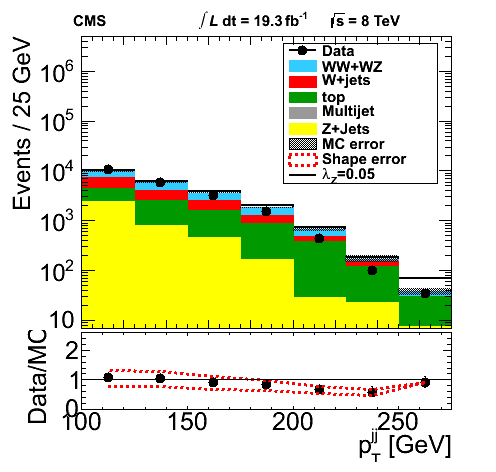
\includegraphics[width=0.48\textwidth]{figs/mu_dijet_dijetPt.png}
    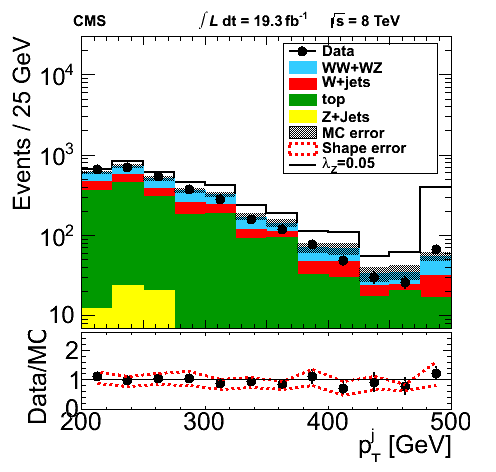
\includegraphics[width=0.48\textwidth]{figs/mu_boosted_dijetPt.png}
    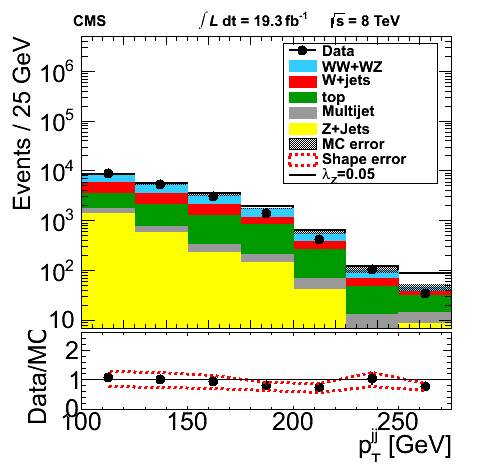
\includegraphics[width=0.48\textwidth]{figs/el_dijet_dijetPt.png}
    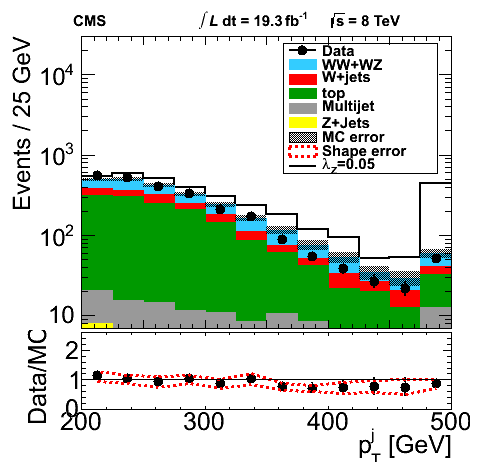
\includegraphics[width=0.48\textwidth]{figs/el_boosted_dijetPt.png}
    \caption{Comparison of the hadronic W $p_T$ distribution using the event 
    selection criteria described in section~\ref{sec:reco}, and with the requirement
    $70 < m_{jj} < 100$~\GeV : 
    muon dijet (upper left), muon boosted (upper right), electron 
    dijet (lower left), electron boosted (lower right).
    The individual components are normalized according to the fit 
    results of section~\ref{sec:mjj_fit} for the $p_T$ range being plotted.}
    \label{fig:ww_dijetPt_stacked}}
\end{figure}
%%%%%%%%%%%%%%%%%%%%%%%%%%%%
%%%%%%%%%%%%%%%%%%%%%%%%%%%%%
We use the ``Higgs Combination'' package \cite{cite:combine} for
setting exclusion limits. This package is a
RooStats\cite{cite:roostats}-based statistical analysis tool-set
recommended by the CMS Higgs PAG and approved by CMS statistics committee.

The coupling parameter space is sampled in a grid around the SM value
of ($\lambda_Z$,$\Delta{\kappa_\gamma}$,$\Delta{g_{1}^Z}$)=(0,0,0) as
described in Sec.~\ref{sec:reweight}. For each of these grid points,
we take as inputs the hadronic W $p_T$ distributions for the
respective signal model, data, and total background that survive after
analysis cuts.  All of these distributions are segregated by lepton
flavor and jet content, which represent independent channel inputs to
the limit setter.  We supply these distributions over the range
$XX-YYY~\gev$ in the form of histograms to the limit setter.

Because of the existence of an interference term (I) in the Lagrangian
between SM background ($B$) and aTGC signal ($S$), this complicates
the evaluation of likelihoods in the signal plus background (plus
interference) hypothesis ($S+B+I$). Such evaluation typically involves
the concept of a signal strength parameter $\mu$, but in this case the
interference effect is not linear with $\mu$. So rather than maximizing
for $\mu$, we perform hypothesis tests involving two alternative signal
models, one that includes aTGC, and one that does not. For each grid point,
the limit setter is set to throw random pseudo-experiments, forming
for each a test statistic that is a ratio of profiled likelihoods

\begin{equation}
q = -2 \ln\frac{{\cal{L}}(data|S_A+B,\hat{\pmb{\theta_A}})}{{\cal{L}}(data|S_0+B,\hat{\pmb{\theta_0}})}
\end{equation}

where in this case the signal strength $\mu$ is fixed to 1 for both
signals $S_A$ (the alternate hypothesis including aTGC and therefore
interference) and $S_0$ (representing the null hypothesis with a
signal equal to the SM WW production). The likelihoods are maximized
individually for each of the nuisance parameters in the set
$\pmb{\theta}$, (the systematic uncertainties described in
Sec.~\ref{sec:syst} comprise this set), $\hat{\pmb{\theta_H}}$
representing the values of $\pmb{\theta}$ that maximize $\cal{L}$ for
the given hypothesis H. ``Data'' in this equation can refer either to
pseudo-experiments, which yields expected limits plus quantiles $\pm$1
and 2~$\sigma$, or the observed data, which yields an observed
limit. P-values for either the $S_0+B$ pseudo-experiment distribution
or observed data are evaluated using the $S_A+B$ distribution, and
then contours in the 2-D space of chosen coupling parameters are
constructed at a value of $p=0.05$, yielding ``$CL_{s+b}$'' limits at
95\% confidence. The resulting limits are plotted.
%%%%%%%%%%%%%%%%%%%%%%%%%%%%%%
%%%%%%%%%%%%%%%%%%%%%%%%%%%%%%
%%%%%%%%%%%%%%%%%%%%%%%%%%%%%%
%%%%%%%%%%%%%%%%%%%%%%%%%%%%%%
\subsection{Systematic uncertainties considered for limit settings}
We considered the following sources of systematics.
%%%%%%%%%%%%%%%%%%%%%%%%%%%%%%%%%%%%%%%%%%%%
\subsubsection{Normalization of the standard model processes}
The uncertainty in the normalization of the sum of the standard model backgrounds 
(diboson, W+jets, $\ttbar$,  single top, QCD multi-jets, and Z+jets processes) 
is taken directly from the diboson signal extraction fit, as 
documented in section~\ref{sec:syst}.
%%%%%
\subsubsection{Normalization of the aTGC cross section}
Since we model the aTGC process via a differential ratio 
(in dijet $p_T$) relative to the standard model process, 
the cross section uncertainty is already accounted for in 
the normalization of the background. 
%%%%%%%%%%%%%%%%%%%%%%%%%%%%
\subsubsection{Luminosity uncertainty}
The latest recommendation for the uncertainty on LHC luminosity is 2.2$\%$~\cite{lumiPAS}.
We propagate LHC luminosity uncertainty of 2.2$\%$~\cite{lumiPAS} 
to the expected yield of the aTGC signal.
%%%%%%%%%%%%%%%%%%%%%%%%%%%%
\subsubsection{Lepton selection and trigger efficiency}
Systematic uncertainties in the trigger efficiencies in
Section~\ref{sec:Eff} are of the order of 1\%. Systematic
uncertainties in the lepton reconstruction and identification
efficiency scale factors are of the order of 2\%. 
%%%%%%%%%%%%%%%%%%%%%%%%%%%%
\subsubsection{Background shape uncertainty}
 The shape uncertainty of the W+jets background 
constitutes a systematic uncertainty. The alternative 
W+jets samples described in Sections~\ref{sec:wjetsShape}-\ref{sec:mjj_fit} 
do not have decent statistics in the tail of high dijet $p_T$ regime. 
Therefore, we take the variation in factorization/renormalization scale 
from MCFM LO. 
Using the same scale choice as used in our default MadGraph sample 
($q_0^2 = M_W^2 + p_{T, W}^2$), we generated samples with 
$q= 2~q_0$ and $q= 0.5~q_0$. 
We then take the maximal variation in the dijet $p_T$ shape with respect 
to the $q= q_0$ as a systematic uncertainty. 
The dijet $p_T$ spectrum has statistically insignificant variation 
when one includes background events with higher jet multiplicity 
(\textit{i. e.}, $\text{N}_{\text{jets}} >2$). 
Figure~\ref{fig:ww_dijetPt_stacked} shows the combined effect of this 
shape systematics.
%%%%%%%%%%%%%%%%%%%%%%%%%%%%
\subsubsection{Signal shape uncertainty}
Since the signal shape is derived from the 
NLO generator at the matrix-element level, the effect of 
factorization/renormalization scale is minuscule.
We verify this for a few aTGC points and assume 
this systematics to be negligible.
%%%%%%%%%%%%%%%%%%%%%%%%%%%%%%
\subsubsection{MCFM signal shape uncertainty due to reweighting}
In order to estimate the uncertainty coming from the reconstruction effects we 
compare the (aTGC/SM) ratios at the generator level and the (aTGC/SM) ratios at 
the reco level after all major selection cuts were applied for both generated and 
reconstructed \textsc{MadGraph} events. Fig.~\ref{fig:correction} 
shows these ratios for samples with different statistics; black and red distributions
correspond to weighted average of several samples for different aTGCs with low statistics 
(i.e. for small values of $\Delta\kappa_{Z},\lambda$ and $\Deltag_{1}^{Z}$). The 
green distribution correspond to a sample with high statistics for which $\Delta\kappa_{\gamma}=+0.5$. 
The ratio is consistent with one and thus, only the statistical error on the ratio 
is taken and propagated as uncertainty on modeling of different aTGC grid points.     
%\begin{equation}
%{aTGC}_{Reco,MadGraph} = (\frac{aTGC}{SM})_{Gen,MCFM}\times\frac{(aTGC/SM)_{Reco, MadGraph}}{(aTGC/SM)_{Gen, MadGraph}}
%\label{corrFormulae}
%\end{equation}

\begin{figure}[h!t]
  {\centering
    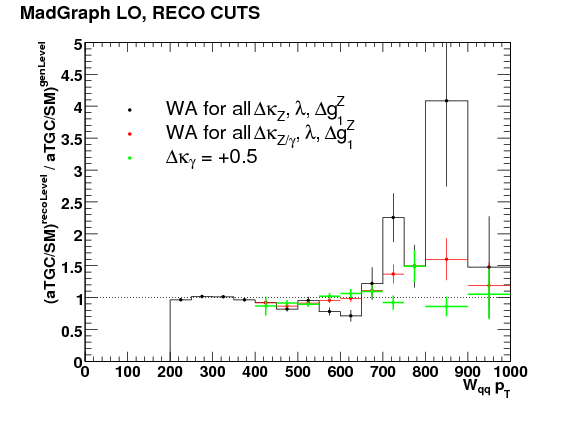
\includegraphics[width=0.6\textwidth]{figs/myfigs/fit-dk-dl-g1z.png}
    \caption{The (aTGC/SM) ratio of reconstructed and generated $WW$ events after selection.}
    \label{fig:correction}}
\end{figure}

%%%%%%%%%%%%%%%%%%%%%%%%%%%%%%
%%%%%%%%%%%%%%%%%%%%%%%%%%%%%%
%%%%%%%%%%%%%%%%%%%%%%%%%%%%%%


%%%%%%%%%%%%%%%%%%%%%%%%%%%%%%
\subsection{Shape-based limit using full \texorpdfstring{19.3 fb${}^{-1}$}{19.5/fb} data sample}
In Fig.~\ref{fig:atgclimits} we present shape-based exclusion limits
on the ATGC parameters. The three possible pair-wise combination of
parameters are considered, assuming the third parameter is set to
zero.  Also, a two-sided limit for each parameter individually is
also presented, assuming the other two parameters are set to
zero. These exclusion limits are computed at the 95\% C.L.

We obtain the following observed exclusion limits:

%% Expected: \\
%% \hspace*{6 mm} $ -0.100 < \, \, \lambda_Z \, \, < 0.086$  \, \, \,(assuming $\Delta{\kappa_\gamma}=0$)\\ 
%% \hspace*{6 mm} $ -0.315 < \, \, \Delta{\kappa_\gamma} \, \, < 0.349$  \, \, \,(assuming $\lambda_Z=0$)\\
%% Observed: \\ 
%% \hspace*{6 mm} $ -0.038 < \, \, \lambda_Z \, \, < 0.03$  \, \, \, (assuming $\Delta{\kappa_\gamma}=0$) \\
%% \hspace*{6 mm} $ -0.11 < \, \, \Delta{\kappa_\gamma} \, \, < 0.14$  \, \, \, (assuming $\lambda_Z=0$).
\hspace*{6 mm} $ -0.013 < \, \, \lambda_Z \, \, < 0.011$  \, \, \, (assuming $\Delta{\kappa_\gamma}=\Delta{g_1^Z}=0$) \\
\hspace*{6 mm} $ -0.042 < \, \, \Delta{\kappa_\gamma} \, \, < 0.062$  \, \, \, (assuming $\lambda_Z=\Delta{g_1^Z}=0$) \\
\hspace*{6 mm} $ -0.012 < \, \, \Delta{g_1^Z} \, \, < 0.031$ \, \, \, (assuming $\lambda_Z=\Delta{\kappa_\gamma}=0$) \\

These limits are consistent with the SM prediction. 
%%%%%%%%%%%%%%%%%%%
%%%%%%%%%%%%%%%%%%%
\begin{figure}[bthp]
\begin{center}
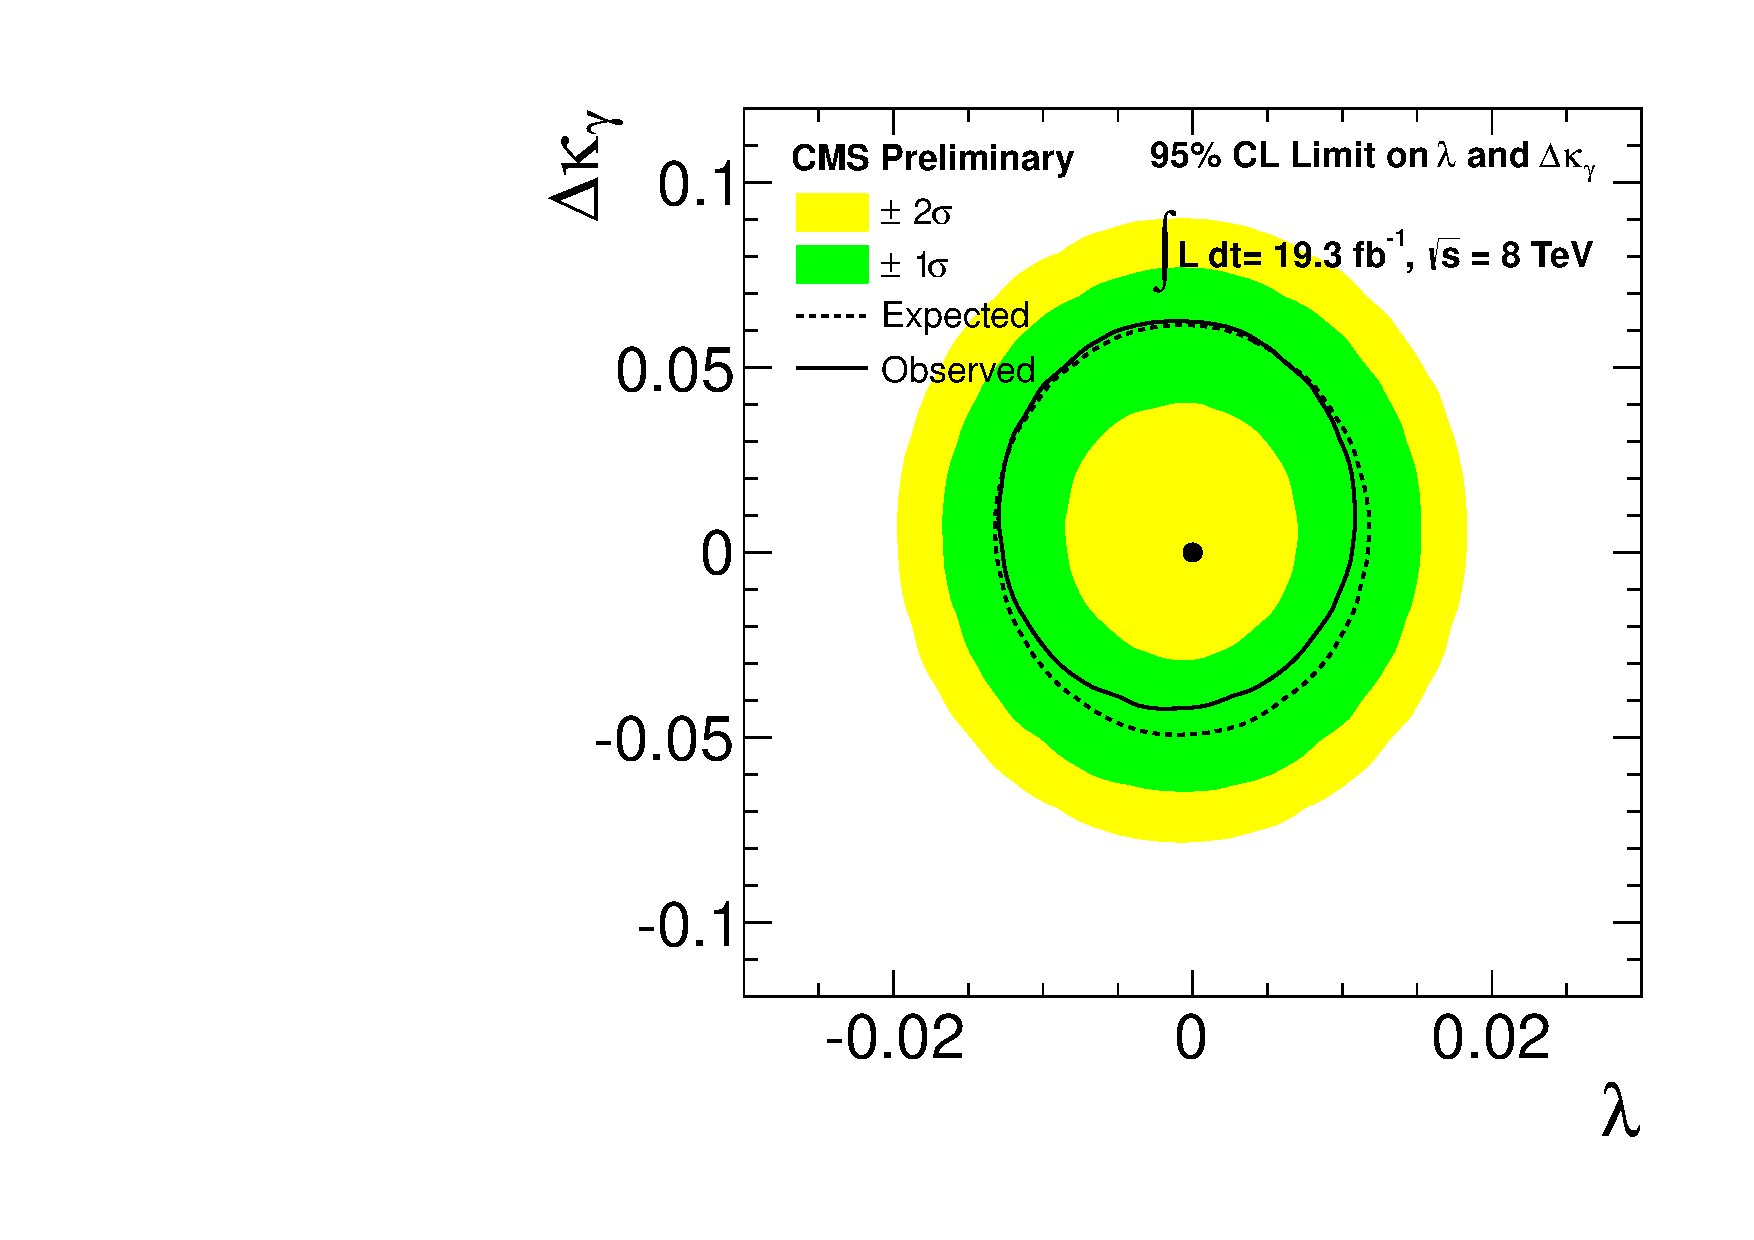
\includegraphics[width=0.45\textwidth]{figs/lz_dkg_2dlimit_Other.pdf}
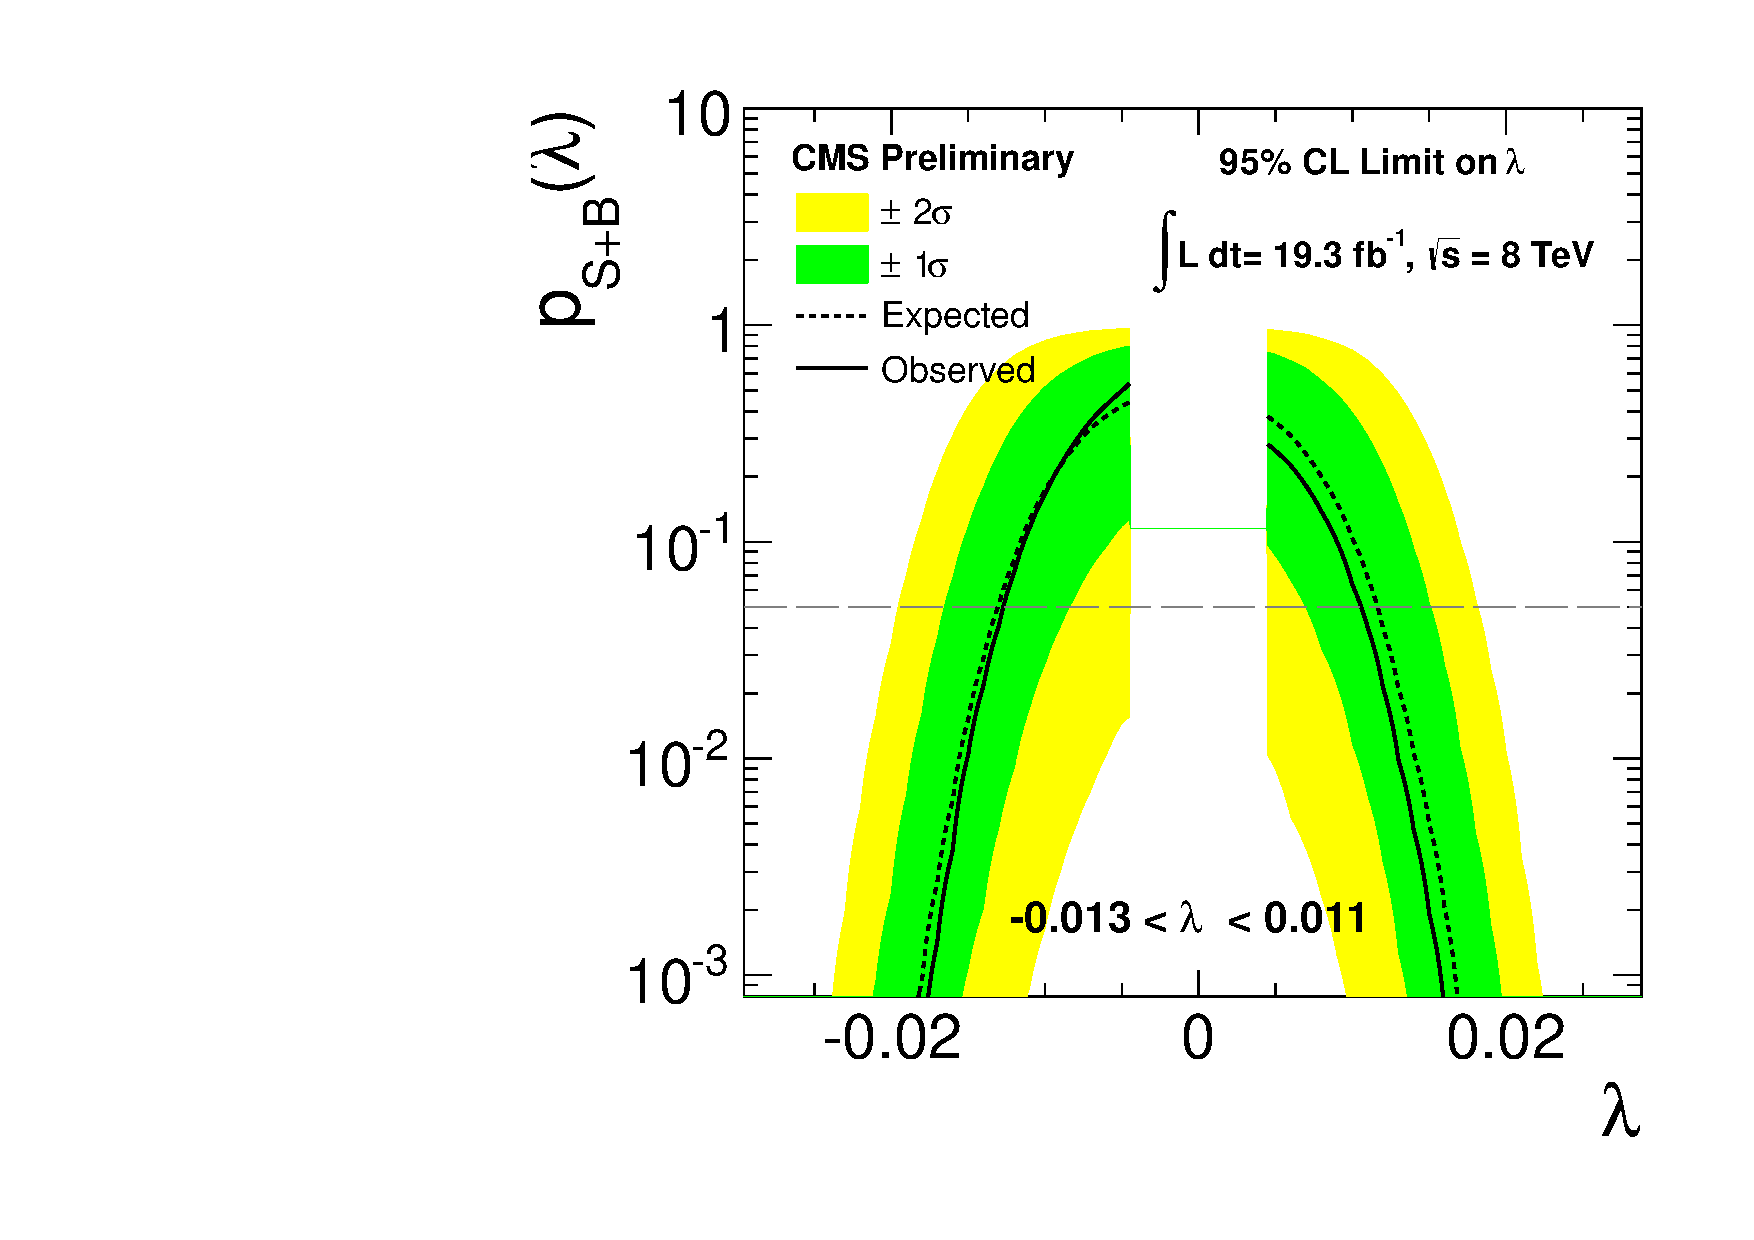
\includegraphics[width=0.45\textwidth]{figs/lz_1dlimit_Other.pdf}
\\
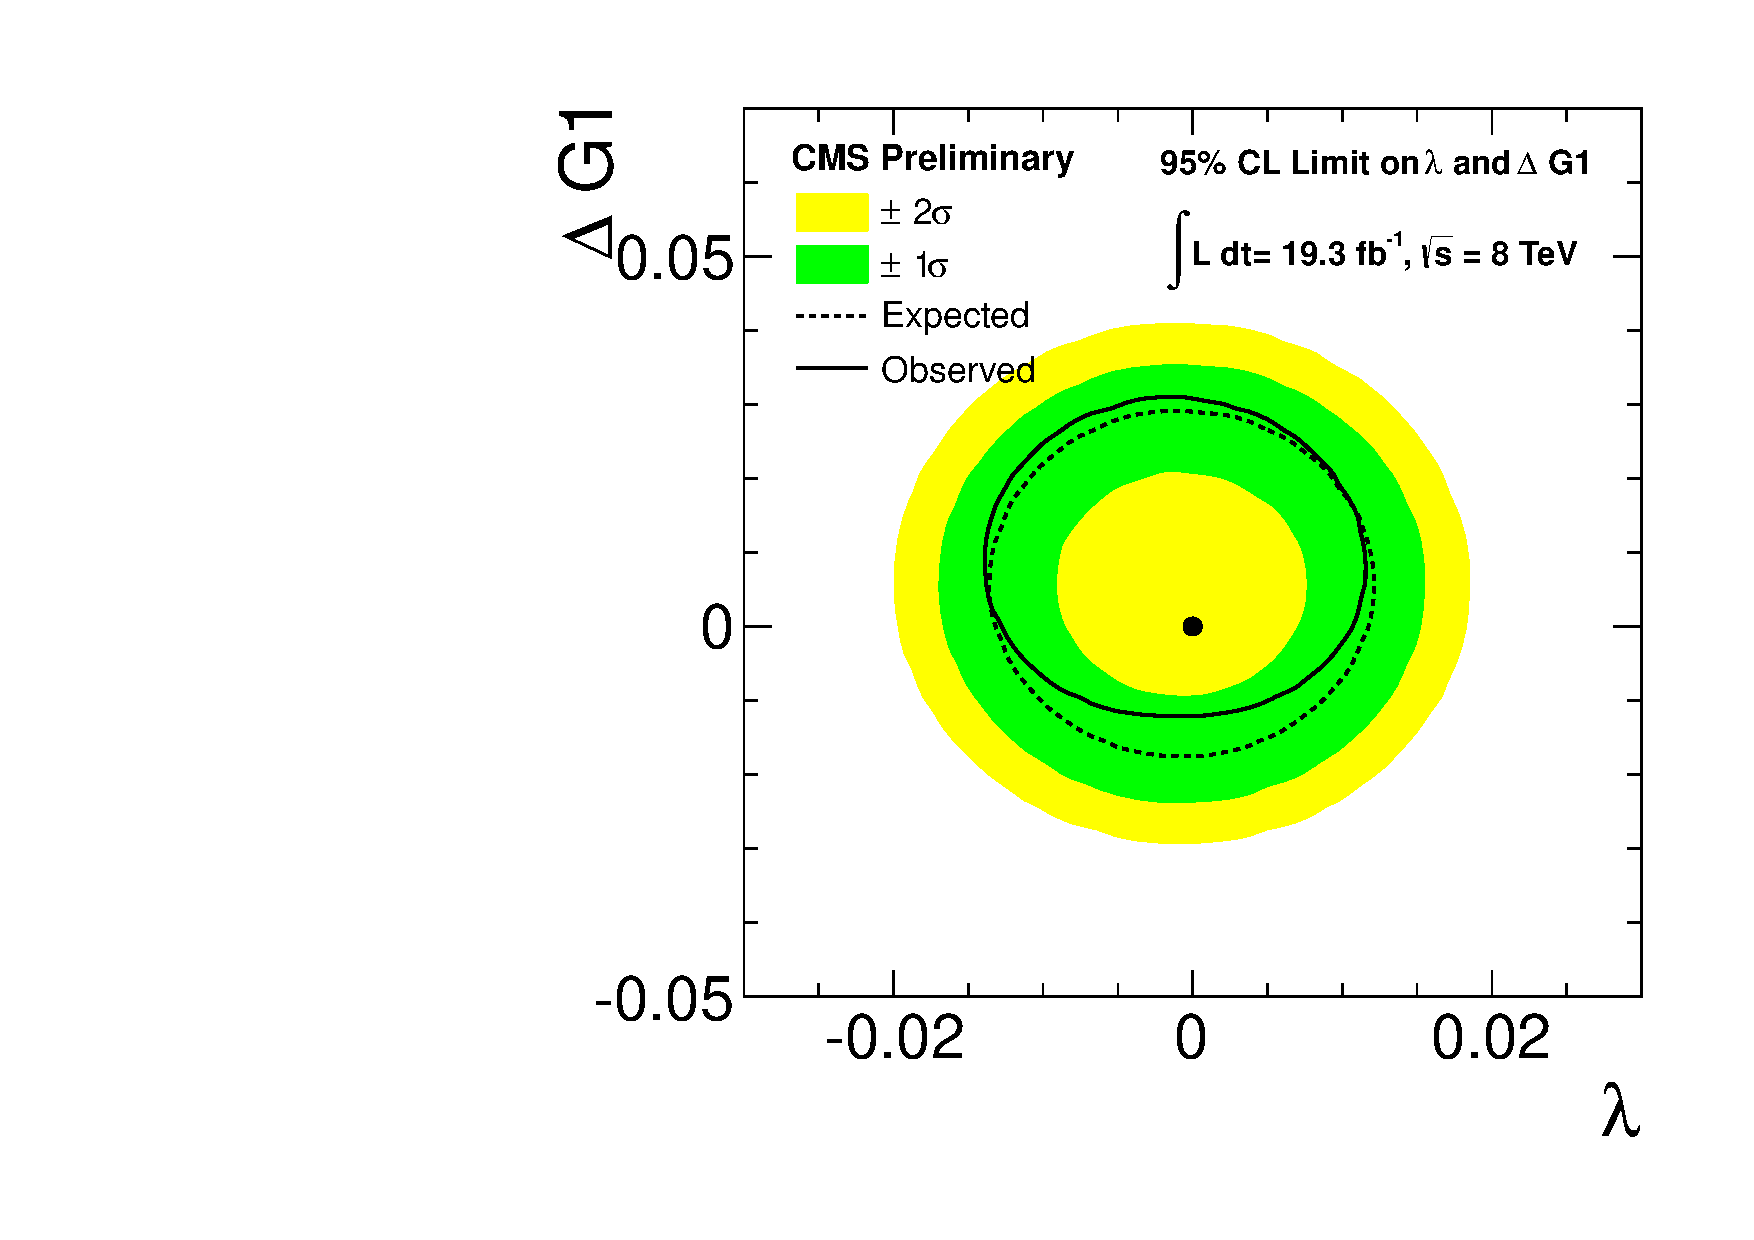
\includegraphics[width=0.45\textwidth]{figs/lz_dg1_2dlimit_Other.pdf}
\includegraphics[width=0.45\textwidth]{figs/dkg_1dlimit_Other.pdf}
\\
\includegraphics[width=0.45\textwidth]{figs/dkg_dg1_2dlimit_Other.pdf}
\includegraphics[width=0.45\textwidth]{figs/dg1_1dlimit_Other.pdf}
\caption{\label{fig:atgclimits}
The observed and expected values of the shape-based limits for 
anomalous triple gauge couplings.
}
\end{center}
\end{figure}
%%%%%%%%%%%%%%%%%%%

%%%%%%%%%%%%%%%%%%%%%%%%%%%%
%%%%%%%%%%%%%%%%%%%%%%%%%%%%%
%\subsubsection{Understanding the limits}

%In order to understand the behavior of our limits we perform a simple 
%Poisson $\chi^{2}$ fit derived from the log-likelihood ratio as:
%\begin{equation}
%  \begin{array}{ccl}
%  \chi^2 = 2\sum_{i}[(p_{i}-d_{i})-d_{i}ln(p_{i}/d_{i})],
%  \label{eq:llr}
%  \end{array}{}
%  \end{equation}
%where $i$ is an aTGC bin, $p_{i}$ is a number of SM 
%events in a bin $i$, and $d_{i}$ is a number of events in a presence 
%of aTGCs in a bin $i$. Clearly, $p_{i}$ is always the same for each aTGC 
%bin. For simplicity, we disregarded the background contibution. We calculate 
%the $\chi^{2}$ values for each aTGC point and their values are shown in 
%Fig.~\ref{fig:chi2}.

%\begin{figure}[h!t]
%  {\centering
%    \includegraphics[width=0.48\textwidth]{figs/myfigs/kappaChi2_1d.png}
%    \includegraphics[width=0.48\textwidth]{figs/myfigs/KappaLambdaChi2.png} \\
%    \includegraphics[width=0.48\textwidth]{figs/myfigs/lambdaChi2_1d.png} 
%    \includegraphics[width=0.48\textwidth]{figs/myfigs/LambdaG1ZChi2.png} \\
%    \includegraphics[width=0.48\textwidth]{figs/myfigs/g1zChi2_1d.png} 
%    \includegraphics[width=0.48\textwidth]{figs/myfigs/KappaG1ZChi2.png} \\
%    \caption{}
%    \label{fig:chi2} The $chi^2$ for each aTGC point.}
%\end{figure}

%The one dimensional distributions of $\chi^{2}$ calculated in this simple way 
%(set of plots on the left side) indicate that 68\% and 95\% C.L. one dimensional 
%limits (marked by the horizontal dashed line for which $\chi^{2}\approx 4$) for 
%$\kappa_{\gamma}$ and $\lambda$ 
%will not be sensitive to the second minimum which appears due to the asymmetry of 
%these cross section relative to the SM. On the contrary, $g_{1}^{Z}$ limits will 
%be sensitive to it as indicated by the left bottom plot. Similar indications are 
%observed for two dimensional limits.


%%%%%%%%%%%%%%%%%%%%%%%%%%%%


\clearpage
